%%%%%%%%%%%%%%%%%%%%%%%%%%%%%%%
%This is the article LaTeX template for RSC journals
%Copyright The Royal Society of Chemistry 2010
%%%%%%%%%%%%%%%%%%%%%%%%%%%%%%%


\documentclass[8.5pt,twoside,twocolumn]{article}
\oddsidemargin -1.2cm
\evensidemargin -1.2cm
\textwidth 18cm
\headheight 1.0in
\topmargin -3.5cm
\textheight 22cm
\usepackage[super,sort&compress,comma]{natbib} 
\usepackage{mhchem}
\usepackage{times,mathptmx}
%\usepackage{times}
% feel free not to use mathptmx if it causes difficulties
\usepackage{sectsty}
\usepackage{balance} 

\usepackage{amsmath}
\usepackage{amssymb}
\usepackage{float}
\newcommand{\e}[1]{\times10^{#1}}
\newcommand{\gd}{\dot{\gamma}}
\newcommand{\com}[1]{{\bf {#1}}}

\usepackage{graphicx} %eps figures can be used instead
\usepackage{lastpage}
\usepackage[format=plain,justification=raggedright,singlelinecheck=false,font=small,labelfont=bf,labelsep=space]{caption} 
\usepackage{fancyhdr}
\pagestyle{fancy}

\begin{document}

\thispagestyle{plain}
\fancypagestyle{plain}{
\fancyhead[L]{
\includegraphics[height=8pt]{headers/LH}}
\fancyhead[C]{\hspace{-1cm}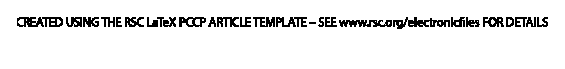
\includegraphics[height=20pt]{headers/CH}}
\fancyhead[R]{
\includegraphics[height=10pt]{headers/RH}\vspace{-0.2cm}}
\renewcommand{\headrulewidth}{1pt}}
\renewcommand{\thefootnote}{\fnsymbol{footnote}}
\renewcommand\footnoterule{\vspace*{1pt}% 
\hrule width 3.4in height 0.4pt \vspace*{5pt}} 
\setcounter{secnumdepth}{5}



\makeatletter 
\def\subsubsection{\@startsection{subsubsection}{3}{10pt}{-1.25ex plus -1ex minus -.1ex}{0ex plus 0ex}{\normalsize\bf}} 
\def\paragraph{\@startsection{paragraph}{4}{10pt}{-1.25ex plus -1ex minus -.1ex}{0ex plus 0ex}{\normalsize\textit}} 
\renewcommand\@biblabel[1]{#1}            
\renewcommand\@makefntext[1]% 
{\noindent\makebox[0pt][r]{\@thefnmark\,}#1}
\makeatother 
\renewcommand{\figurename}{\small{Fig.}~}
\sectionfont{\large}
\subsectionfont{\normalsize} 

\fancyfoot{}
\fancyfoot[LO,RE]{\vspace{-7pt}
\includegraphics[height=9pt]{headers/LF}}
\fancyfoot[CO]{\vspace{-7.2pt}\hspace{12.2cm}
\includegraphics{headers/RF}}
\fancyfoot[CE]{\vspace{-7.5pt}\hspace{-13.5cm}
\includegraphics{headers/RF}}
\fancyfoot[RO]{\footnotesize{\sffamily{1--\pageref{LastPage} ~\textbar  \hspace{2pt}\thepage}}}
\fancyfoot[LE]{\footnotesize{\sffamily{\thepage~\textbar\hspace{3.45cm} 1--\pageref{LastPage}}}}
\fancyhead{}
\renewcommand{\headrulewidth}{1pt} 
\renewcommand{\footrulewidth}{1pt}
\setlength{\arrayrulewidth}{1pt}
\setlength{\columnsep}{6.5mm}
\setlength\bibsep{1pt}

\twocolumn[
  \begin{@twocolumnfalse}
\noindent\LARGE{\textbf{Rheology of Cubic Blue Phases}}
\vspace{0.6cm}

\noindent\large{\textbf{Oliver Henrich $^{\ast}$\textit{$^{a,b}$}, Kevin Stratford \textit{$^{a}$}, Peter V. Coveney \textit{$^{b}$}, Michael E. Cates \textit{$^{c}$}, Davide Marenduzzo \textit{$^{c}$}}}\vspace{0.5cm}
%Please note that \ast indicates the corresponding author(s) but no footnote text is required. 


\noindent\textit{\small{\textbf{Received Xth XXXXXXXXXX 20XX, Accepted Xth XXXXXXXXX 20XX\newline
First published on the web Xth XXXXXXXXXX 200X}}}

\noindent \textbf{\small{DOI: }}
\vspace{0.6cm}
%Please do not change this text.

\noindent \normalsize{We study the behaviour of cubic blue phases under shear flow 
via lattice Boltzmann simulations. We focus on the two experimentally observed
phases, Blue Phase I (BPI) and Blue Phase II (BPII). The disclination network of Blue Phase 
II continuously breaks and reforms under steady shear, leading to an oscillatory stress response in time.
For larger shear rates, the structure breaks up into a cholesteric helix, lying either along the
vorticity or the flow gradient direction according to the imposed flow.
BPI leads to a very different response. Here, oscillations are only possible for intermediate
shear rates -- very slow flow leads to a transition into an amorphous network 
with an apparent yield stress. The flow-induced oscillation regime features a novel arrangement
of double helical disclinations which rotate due to the shear. Large flow rates can, 
just as in the BPII case, lead to the rupture of the network and the stabilisation
of less ordered cholesteric structures. Our results provide the first 
theoretical investigation of sheared blue phases in large systems, and
are relevant to understanding the bulk rheology of these materials.}
\vspace{0.5cm}
 \end{@twocolumnfalse}
  ]

%\footnotetext{\dag~Electronic Supplementary Information (ESI) available: [details of any supplementary information available should be included here]. See DOI: 10.1039/b000000x/}

%Please use \dag to cite the ESI in the main text of the article.
%If you article does not have ESI please remove the the \dag symbol from the title and the above footnotetext.

\footnotetext{\textit{$^{a}$~EPCC, School of Physics and Astronomy, University of Edinburgh,\\JCMB Kings Buildings, Mayfield Road, Edinburgh EH9 3JZ, UK; E-mail: ohenrich@epcc.ed.ac.uk}}
\footnotetext{\textit{$^{b}$~Centre for Computational Science, University College London,\\20 Gordon Street, London WC1H 0AJ, UK}}
\footnotetext{\textit{$^{c}$~SUPA, School of Physics and Astronomy, University of Edinburgh,\\JCMB Kings Buildings, Mayfield Road, Edinburgh EH9 3JZ, UK}}

%additional addresses can be cited as above using the lower-case letters, c, d, e... If all authors are from the same address, no letter is required

%\footnotetext{\ddag~Additional footnotes to the title and authors can be included \emph{e.g.}\ `Present address:' or `These authors contributed equally to this work' as above using the symbols: \ddag, \textsection, and \P. Please place the appropriate symbol next to the author's name and include a \texttt{\textbackslash footnotetext} entry in the the correct place in the list.}


\section{Introduction}
% Put \label in argument of \section for cross-referencing
%\section{\label{}}

Cholesterics are liquid crystals in which the local nematic director field shows spontaneous 
twist in thermodynamic equilibrium~\cite{deGennes}. 
The simplest manifestation is the standard cholesteric phase where the
director precesses around a single helical axis of fixed orientation.
For highly chiral systems, however,
the preferred configuration close 
to the isotropic boundary features twist around two perpendicular axes, as opposed to 
just one axis in the regular cholesteric state, and the corresponding deformation is 
denoted a ``double-twist cylinder''.
As it is topologically impossible to cover continuously 3D space with double-twist 
cylinders, defects arise. The resulting disclination lines (at which the
nematic director is undefined)
 organise into a variety of regular periodic lattices, 
giving rise to the so-called cubic blue phases (BPs)~\cite{Grebel:1984,Wright:1989}. 
There are two experimentally observed cubic blue phases, BPI and BPII (a third, BPIII, 
is thought to be amorphous~\cite{Henrich:2011a}).

BPs were long considered as purely of academic interest due to their very narrow 
range of stability. This view has changed since the creation of polymer-stabilised and other thermally 
stabilised BPs~\cite{Kikuchi:2002,Coles:2005}, which has opened up the 
possibility of novel applications.
During the last few years considerable progress has been achieved regarding the behaviour 
of BPs in confined geometries~\cite{Fukuda:2010a, Fukuda:2010b, Ravnik:2011b}, under 
external fields~\cite{Alexander:2008,Fukuda:2009,Henrich:2010a,Castles:2010,Tiribocchi:2011a}, 
and in the presence of colloidal particles~\cite{Ravnik:2011a}.
The kinetics of BP domain growth have been recently addressed~\cite{Henrich:2010b}. 
However, our understanding of their dynamical behaviour under flow remains
very limited. The aim of this work is to address this issue by studying,
for the first time, the response of large BP samples to a shear flow.

Flow response in cholesterics is both strongly non-Newtonian and highly anisotropic.
For example, if a standard cholesteric phase is subjected to a Poiseuille flow along
its helical axis, small pressure differences drive flow mainly through
``permeation'', as first investigated by Helfrich~\cite{Helfrich:1969}.
In the permeation mode the liquid crystal flows while leaving the director
field virtually unchanged, which leads to high dissipation and large
viscosities. Marenduzzo et al.~\cite{Marenduzzo:2006a,Marenduzzo:2006b} simulated 
shear and Poiseuille flow in cholesteric liquid crystals in the permeation mode, and 
showed the importance of the boundary conditions in determining the apparent viscosity of the fluid. 
They also found that a strong secondary flow appears.
Rey~\cite{Rey:1996a, Rey:1996b} studied shear in cholesterics oriented with the helix along 
the vorticity axis and found that, at low Ericksen number, travelling twist waves appear which 
lead to the rotation of the cholesteric helix. At higher forcing, the helix uncoils, creating a flow-induced nematic phase.
Rey also studied cholesterics subjected to both steady flow and low frequency
small amplitude oscillatory shear for different helix orientations
~\cite{Rey:2000, Rey:2002}. He found that splay/bend/twist deformations were
excited when the helix was aligned along the flow direction; splay/bend
deformation occurred when the helix was aligned along the velocity gradient;
but only twist deformations
appeared when the helix was aligned along the vorticity axis.

Dupuis et al.~\cite{Dupuis:2005} performed the first numerical investigation of BP rheology 
in Poiseuille flow, starting from equilibrium structures of BPI and BPII and a periodic 
array of doubly twisted cylinders.
Under small forcing, the network opposed the flow, giving rise to a significant 
increase in apparent viscosity.
Upon increasing the forcing they found clear evidence of shear thinning.
In the crossover region they predicted a novel oscillatory regime where the network 
continuously breaks and reforms as portions of the disclinations in the centre of the channel 
move to neighbouring cells and relink with the parts of the network left behind by the flow. 
The viscosity still decreases with forcing 
(the system shear thins) but much less than
for cholesterics in the permeation mode, which is in agreement with experiments
~\cite{Zapotocky:1999, Ramos:2002}.

Our work differs from these earlier efforts as it addresses homogeneous shear flows, 
and focuses on flow-induced reconstruction and nonequilibrium transition
between different blue phase networks, which appear at intermediate or
high shear. Our simulations employ Lees-Edwards boundary conditions, which
are naturally suited to address these regimes, and bulk as opposed
to boundary-dominated flow. 
Our simulations are large scale and parallel, so that we can study
significantly larger systems than previously possible, and our
results can in principle be compared with bulk rheology experiments. 

Our paper is organised as follows. 
In Section II, we describe the method we use and review
the hydrodynamic equations of motion which we aim to solve. In Section III, 
we report our numerical results, separating them into subsections referring to
Blue Phase I and Blue Phase II, and corresponding to low, intermediate, and
high shear. Finally, we draw our conclusions in Section IV.

\section{Model and Methods}

Our approach is based on the well-established Beris-Edwards model for hydrodynamics of
cholesteric liquid crystals \cite{Beris:1994}, which describes the ordered state 
in terms of a traceless, symmetric tensor order parameter ${\mathbf Q}({\mathbf r})$. 
In the uniaxial approximation, the order parameter is given by
$Q_{\alpha \beta}= q_s ( \hat{n}_\alpha \hat{n}_\beta - \frac{1}{3}\; \delta_{\alpha\beta})$
with $\hat{{\mathbf n}}$ the director field and $q_s$ the amplitude of nematic
order. More generally,
the largest eigenvalue of ${\mathbf Q}$, $0\le q_s\le\frac{2}{3}$
characterises the local degree of orientational order.
The thermodynamic properties of the liquid crystal are determined by a free energy
${\cal F}$, whose density $f$ consists of a bulk contribution $f_b$ and a gradient part $f_g$, as follows,
\begin{eqnarray}
f_b&=&\frac{A_0}{2}\left(1-\frac{\gamma}{3}\right) Q_{\alpha \beta}^2\nonumber\\
&-&\frac{A_0 \gamma}{3}Q_{\alpha \beta} Q_{\beta \gamma} Q_{\gamma \alpha}+\frac{A_0 \gamma}{4}(Q_{\alpha \beta}^2)^2,\nonumber\\
f_g&=&\frac{K}{2}(\varepsilon_{\alpha\gamma\delta} \partial_\gamma Q_{\delta\beta}+2 q_0 Q_{\alpha \beta})^2+\frac{K}{2}(\partial_\beta Q_{\alpha \beta})^2.\label{FE}
\end{eqnarray}
The first term contains a bulk-free energy constant $A_0$ and the temperature-related parameter $\gamma$ which controls the magnitude of order.
The second part quantifies the cost of elastic distortions, which is proportional to the elastic constant $K$;
we work for simplicity in the one-elastic constant approximation~\cite{deGennes}. The wavevector $q_0$ is equal to $2\pi/p_0$, where $p_0$ is the cholesteric pitch.
The actual periodicity of the BP structure, $p$, does not need to be equal to $p_0$.
Indeed, the ``redshift'' $r=p/p_0$ is adjusted during the equilibration phase of the 
simulation, to optimise the free energy density
before shearing begins -- this is done by following the procedure
previously described in~\cite{Alexander:2006}.

A thermodynamic state is specified by two dimensionless quantities: the reduced temperature 
\begin{equation}
\tau=\frac{27(1-\gamma/3)}{\gamma},
\end{equation}
which vanishes at the spinodal point of a nematic ($q_0=0$), 
and the reduced chirality 
\begin{equation}
\kappa=\sqrt{\frac{108 K q_0^2}{A_0 \gamma}},
\end{equation}
which measures the ratio of gradient to bulk free energy.

The dynamical evolution of the order parameter is given by the equation 
\begin{equation}
\left(\partial_t+ v_\alpha \partial_\alpha \right){\mathbf Q} - {\mathbf S}({\mathbf W},{\mathbf Q}) = \Gamma {\mathbf H}.
\label{op-eom}
\end{equation}
The first term on the left hand side of Eq.\ref{op-eom} is a material derivative, which describes the rate of change of a quantity advected by the flow.
The second term accounts for the rate of change due to local velocity gradients $W_{\alpha \beta}=\partial_\beta v_\alpha$,
and is explicitly given by~\cite{Beris:1994}
\begin{eqnarray}
{\mathbf S}({\mathbf W}, {\mathbf Q}) &=& (\xi {\mathbf A} + {\boldsymbol \Omega})({\mathbf Q}+\frac{\mathbf I}{3})\nonumber\\
& &\hspace*{-1.5cm}+ ({\mathbf Q}+\frac{\mathbf I}{3})(\xi {\mathbf A}  - {\boldsymbol \Omega})-2 \xi ({\mathbf Q}+\frac{\mathbf I}{3})
\mathrm{Tr}({\mathbf Q W}),
\label{sw}
\end{eqnarray}
where $\mathrm{Tr}$ denotes the tensorial trace, while 
${\mathbf A}=({\mathbf W}+{\mathbf W}^T)/2$ and
${\boldsymbol \Omega}=({\mathbf W}-{\mathbf W}^T)/2$ are the symmetric and antisymmetric part of the velocity gradient, respectively. $\xi$ 
is a constant depending on the molecular details of the liquid crystal.
Flow alignment occurs if $\xi \cos{2\theta}=(3q_s)/(2+q_s)$ has a real solution for $\theta$, the 
so-called Leslie angle: we select this case by 
setting $\xi=0.7$ in our simulations.
${\mathbf H}$ is the molecular field, which is a functional derivative of $\cal F$ that respects the tracelessness of $\mathbf Q$:
\begin{equation}
{\bf H}=-\frac{\delta {\cal F}}{\delta {\bf Q}}+\frac{\bf I}{3}\,
\mathrm{Tr} \left(\frac{\delta {\cal F}}{\delta {\bf Q}}\right).
\label{molfield}
\end{equation}
The rotational diffusion constant $\Gamma$ in Eq.~\ref{op-eom} is proportional
to the inverse of the rotational viscosity $\gamma_1=2 q_s^2/\Gamma$
\cite{deGennes}.

The time evolution of the fluid density and velocity are respectively governed
by the continuity equation
$\partial_t \rho = -\partial_\alpha(\rho v_\alpha)$, and
the following Navier-Stokes equation:
\begin{eqnarray}
\partial_t v_\alpha +\rho \,v_\beta \partial_\beta v_\alpha
&=& \partial_\beta \Pi_{\alpha \beta}+ \eta\, \partial_\beta [ \partial_\alpha v_\beta +\; \partial_\beta v_\alpha].
\label{NSE}
\end{eqnarray}
This emerges from the Chapman-Enskog expansion
of the lattice Boltzmann (LB) equations 
that we solve numerically. A further term $\eta(1+3\frac{\partial P_0}{\partial\rho} )\partial_\mu v_\mu \delta_{\alpha \beta}$ that formally appears
in this expansion is negligible under the slow flows considered here
for which the the fluid motion is almost incompressible~\cite{Denniston:2001}.
$\eta$ is an isotropic background viscosity which is set to $\eta=0.8333$ in LB units (these are discussed below, see~\cite{Henrich:2011a,Henrich:2010b}).
The thermodynamic stress tensor reads explicitly
\begin{eqnarray}
\Pi_{\alpha \beta}&=&P_0 \delta_{\alpha\beta}
-\xi H_{\alpha \gamma}\left(Q_{\gamma \beta} +\frac{1}{3} \delta_{\gamma \beta}\right)\nonumber\\
&-&\xi \left(Q_{\alpha \gamma} +\frac{1}{3} \delta_{\alpha \gamma}\right) H_{\gamma \beta} + Q_{\alpha \gamma}H_{\gamma \beta}-H_{\alpha \gamma} Q_{\gamma \beta} \nonumber\\
&+&2 \xi  \left(Q_{\alpha \beta} +\frac{1}{3} \delta_{\alpha \beta}\right) Q_{\gamma \nu} H_{\gamma \nu}
- \partial_\alpha Q_{\gamma \nu} \frac{\delta{\cal F}}{\delta \partial_{\beta} Q_{\gamma \nu}}\nonumber\\
\label{Pi}
\end{eqnarray}
and is responsible for strong non-Newtonian flow effects.
In the isotropic state ${\bf Q}\equiv 0$ and Eq.\ref{Pi} reduces to the
scalar pressure as would appear in Eq.~\ref{NSE} for a Newtonian fluid. 

We next define a 
dimensionless number that describes the deformation
of the director field under flow. This so-called Ericksen number
is given by 
\begin{equation}
Er=\frac{\eta v l}{K}
\end{equation}
with $\eta$ and $K$ defined previously, and 
$v$ and $l$ a typical velocity and length scale. 
In the present work $l=p_0/2$ was used as this is the approximate size of
the BP unit cell. Likewise, $v$ was taken to be the velocity difference
across one unit cell, i.e. $v=\dot{\gamma} p_0/2$. 

\if{The spectrum $X_\omega$ of the shear stress $\Pi_{xy}(t)$ was determined via discrete Fourier transformation according to
\begin{equation}
X_\omega=\frac{1}{\sqrt{N}}\sum_{n=0}^{N-1} \left[\Pi_{xy}(t_n) - \bar{\Pi}_{xy}\right] \exp(2\pi i \, \omega \,n\,/\,N),
\label{spectrum}
\end{equation}
where we subtract the average stress $\bar{\Pi}_{xy}$ from the signal.
$N$ was the number of points in the time series, typically one for every 100 LB time steps. }\fi

The system of coupled partial differential equations~\ref{op-eom}
and~\ref{NSE} is solved by means of a hybrid method~\cite{Marenduzzo:2007}
which uses a combination of lattice Boltzmann and finite difference schemes.
(This is in contrast with some earlier methods using solely
LB~\cite{Denniston:2001, Denniston:2004}.)
The Navier-Stokes
equation is solved via the lattice Boltzmann approach, using a standard
three-dimensional model with 19 discrete velocities (D3Q19).
A regular lattice with spacing $\Delta x = \Delta y = \Delta z = 1$ is
used and the time step is $\Delta t = 1$ in lattice units.
Coupling to the thermodynamic sector is via a
local body force computed as the divergence of the thermodynamic
stress Eq.~\ref{Pi}; the resulting velocity field is used in the computation
of the time evolution of $\mathbf{Q}$ via a standard finite difference
method using the same grid and the same time step as the LB. The system
is periodic in all three coordinate directions. Sliding
boundary conditions, or Lees-Edwards planes, are explicitly implemented
in both hydrodynamic and thermodynamic sectors to impose shear on the
system. On
crossing a Lees-Edwards boundary a Galilean transformation is applied
with a velocity increment which is fixed in time (and limited in size by the
low Mach number constraint of LB). An appropriate transformation
of LB distributions which propagate across a boundary~\cite{Wagner:2002}
must be applied at each time step, and appropriate
adjustment to $W_{\alpha\beta}$ is required to compute cross-plane
gradients of the velocity field used in the update to ${\mathbf Q}$.
In both cases interpolation of the
relevant quantities is required to cope with the relative displacement
of neighbouring lattice sites separated by a sliding plane (the
displacement may be a fraction of a lattice unit at any given time
step). The use of multiple sliding planes equally spaced in a single
system allows
the overall shear rate to be maintained indefinitely as the system
becomes larger
in the velocity gradient direction (in contrast with the use of solid
walls to impose shear). This hybrid method with Lees-Edwards planes
has been used successfully to study e.g., smectics~\cite{Henrich:2012a}.


In the following we report results of simulations of the bulk flow behaviour of the cubic blue 
phases BPI and BPII.
Typical runtimes for system size $L_x\times L_y\times L_z=128^3$ on 512 processes were in the region of 18 to 24 hours.  
The timestep and lattice spacing in lattice Boltzmann units (LBU) can be mapped
approximately to $\sim 1 {\rm ns}$ and $\sim 10{\rm nm}$ in SI units, respectively. The LB unit of stress
is equal to about $10^8$~Pa. Further details about the conversion 
from LBU to SI units can be found elsewhere~\cite{Henrich:2011a,Henrich:2010b}.
In what follows, $x$, $y$ and $z$ denote respectively the velocity, velocity
gradient and vorticity direction; $\Pi_{xy}$ is therefore the shear stress.

\section{Results and Discussion}

For typical simulations reported in this work, 
we chose as initial conditions thermodynamic states that are 
well inside the equilibrium region of the individual blue phase, and far away 
from the cholesteric-isotropic transition. Thus, temperature and chirality were 
$\tau=-0.5, \kappa=1.0$ in case of BPI and $\tau=-0.5, \kappa=2.0$ for BPII, respectively.
For these parameters the total free energy density $f$ remained always negative at all flow rates
simulated. 
Since by Eq.~\ref{FE} $f=0$ for an isotropic phase with ${\mathbf Q}\equiv 0$, this means that our system, which is never far from equilibrium locally even under flow, always remains in a liquid crystalline state. 
We also performed selected simulations on metastable states at higher and lower temperatures, 
and at different chiralities, but did not find any significant differences in the 
general flow behaviour from that described below.
The only quantitative difference we found was that, for thermodynamic states that are closer to the phase boundary than the one we focused on (and describe below), the critical shear
rate at which the disclination 
network broke up into chiral nematic states was lower. This is expected as these states have on average higher free energy densities and smaller order parameters than those we focus on in what follows, and cannot therefore withstand the same external forces before breaking down.

As usual in BP simulation studies~\cite{Henrich:2011a,Henrich:2010b}, we initialised our runs with 
analytical solutions that minimise the free energy functional Eq.\ref{FE} in the high-chirality limit 
and equilibrated these configuration for 5000 LB timesteps before we started the shear flow. 
During the equilibration sequence the optimal redshift $r$ was calculated and applied at every timestep.
After equilibration the redshift was kept constant throughout the rest of the simulation with shear flow (as 
it is no longer justified to optimise the free energy in a nonequilibrium scenario).
We chose a pitch length of 32 LBU for BPII and 64 LBU in case of BPI, and we considered in both cases 
4 unit cells along each coordinate direction, for a total of 64 unit cells in our simulation box.
Runs with higher resolution confirmed that this choice was adequate to track  
all kinematic details of the blue phase networks in shear flow. This includes
reconstruction of the unit cell not accessible in simulation with only
few cells~\cite{Dupuis:2005}.

Simple shear flow was imposed by means of the Lees-Edwards boundary
conditions with
the top (bottom) part of the system flowing in the positive (negative) $x$-direction and the 
velocity gradient along the $y$-direction.
The shear rates were varied over more than two orders of magnitude from about 
$\gd=2.44\times \e{-6}$ to $1.875\times\e{-3}$ LBU.
For clarity we classify various flow regimes, two in the case of BPII and three in the 
case of BPI. 
They are BPII-1 ($\gd \lesssim 3.125\e{-4}$, corresponding to ${\it Er} \lesssim 2.67$), 
BPII-2 ($4.687\lesssim \gd\lesssim 6.25\e{-4}$; $4\lesssim {\it Er} \lesssim 5.34$), ),
BPI-1 ($\gd \lesssim 1.95\e{-5}$; ${\it Er} \lesssim 0.33$), ), BPI-2 ($3.91\e{-5}\lesssim \gd \lesssim 4.687\e{-4}$; $0.67\lesssim {\it Er} \lesssim 8$) and BPI-3 ($6.25\e{-4}\lesssim \gd\lesssim 7.813\e{-4}$; $10.67 \lesssim {\it Er} \lesssim 13.33$).
Beyond these regimes, and prior to the ultimate breakdown into an isotropic phase, 
both BPI and BPII form common configurations regardless 
of the initial state. These are a cholesteric helix with helical axis 
oriented along the direction of the velocity gradient (CHG), 
and a flow-aligned nematic state (FAN).  
As is standard \cite{Henrich:2010b,Henrich:2012b} disclination lines are represented by plotting an isosurface of the scalar order parameter $q_s$. 
Typical choices are $q_s=0.18$ for BPI and $q_s=0.15$ for BPII.
(Note that $q_s$ is small but non-zero at the disclination core. The director is undefined there because the largest and second largest eigenvalues of ${\mathbf Q}$ coincide.)

\subsection{Blue Phase II}

\begin{figure}[htpb]
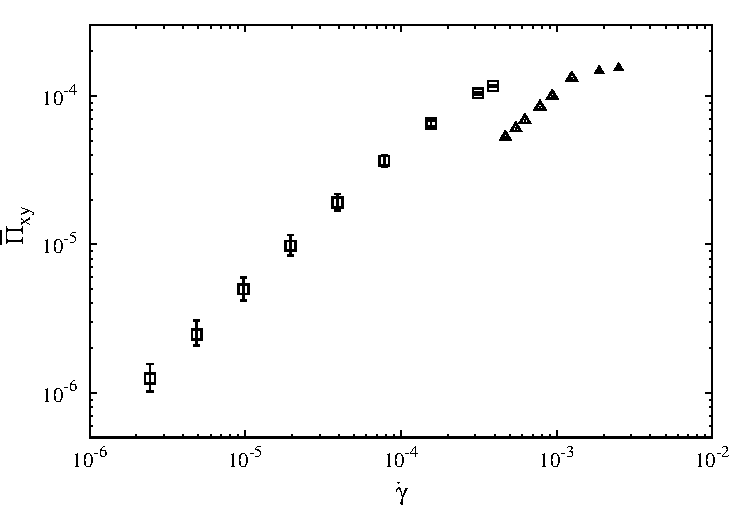
\includegraphics[width=0.495\textwidth]{flowcurve_bp2.pdf}\\
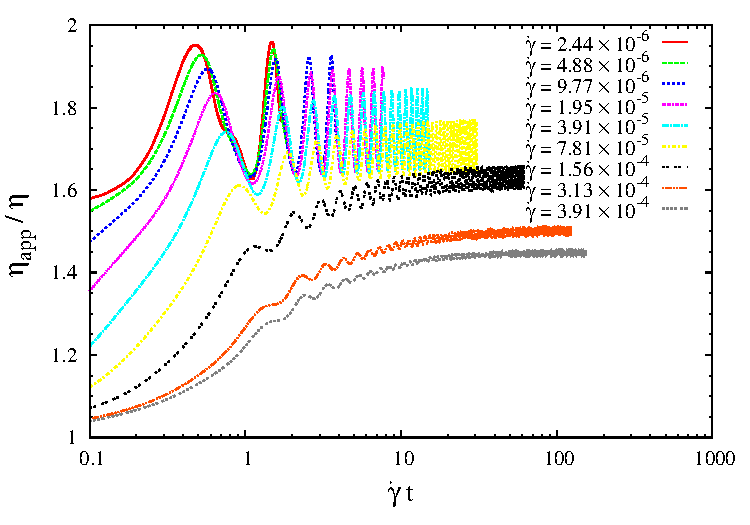
\includegraphics[width=0.495\textwidth]{app_visc_strain_bp2_a.pdf}\\
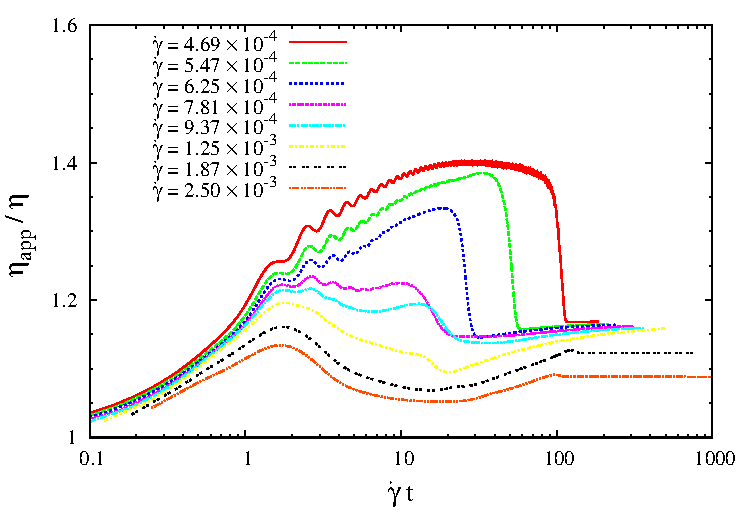
\includegraphics[width=0.495\textwidth]{app_visc_strain_bp2_b.pdf}\\
\caption{Apparent viscosity $\eta_{app}=\Pi_{xy}/\gd$ (normalised to $\eta$) 
of BPII versus time (top) and strain (bottom). 
For clarity the individual curves have been shifted along the time and strain axis. 
The inset in the top panel 
shows the flow curve $\bar{\Pi}_{xy}(\gd)$ and two different regimes of flow: 
regular periodic breakup and reconnecting of the disclination lines (BPII-1, open circles), 
break up of the network into a travelling helical wave (BPII-2, solid circle), 
cholesteric helix with axis in gradient direction (CHG, open squares)
and flow-aligned nematic state (FAN, solid square).
The error bars indicate the maximum and minimum stresses that occur during one cycle.}
\label{bp2-rheo}
\end{figure}

We start our discussion with BPII as its flow behaviour is somewhat simpler 
than that of BPI. BPII has simple cubic symmetry and the disclination lines 
intersect and form a characteristic network of nodes.
Ahead of the more detailed discussion we provide first a general overview of the 
flow behaviour at all applied shear rates.
Fig. \ref{bp2-rheo} shows the ratio between the apparent viscosity, 
defined as 
$\eta_{app}=\langle \Pi_{xy} \rangle/\gd$, and $\eta$.
A numerical value of $\eta_{app}/\eta=1$ corresponds to a fully Newtonian flow,
without any additional contribution from the liquid crystal.
The top picture shows the data over time, whereas the graph at the bottom gives 
the same data versus accumulated strain.
For all but the highest flow rates $\eta_{app}$ oscillates sinusoidally, which
is because of the periodic breakup and reconnecting of the network in shear flow. 
We refer to this regime as BPII-1. As noted in the Appendix, the
absence at very low shear rate of a permeation mode is due to our
choice of boundary conditions.
%{We note that permeation flows, which would
%{\em not} lead to oscillatory response, are effectively disallowed by the combination
%of the geometry and boundary condition we consider. This is
%because the periodic boundary conditions impose macroscopic distortion
%of the network, and are effective analogous to infinitely distant
%but anchored wall along the $xy$ plane.
%This means that  our results are effectively valid for sheared bulk 
%BPs which are anchored at the walls. Furthermore, permeation flows are 
%only restricted to very slow flows, and are unstable for intermediate 
%and high flows, where the response of the network depends less on
%the details of the boundary conditions used at 
%the wall~\cite{Marenduzzo:2006a,Marenduzzo:2006b}.}

The inset to Fig. 1 (top) shows a flow curve, defined as time averages of 
the shear stress $\bar{\Pi}_{xy}$ as a function of shear rate $\gd$.
For all but the largest shear rates a power law fit $\bar{\Pi}_{xy}=a \gd^b$ with 
$a=0.35, b=0.95$ describes the data to a very good approximation. 
Hence, the degree of shear-thinning is remarkably small in BPII, in
the range of shear rates which we have explored here.

For shear rates $4.68\e{-4}\lesssim\gd\lesssim6.25\e{-4}$ ($4\lesssim {\it Er} \lesssim 5.34$) the network of disclination lines
breaks up completely, and oscillations in the stress signal are absent.
In this regime of shear rates, to which we refer as BPII-2, the 
blue phase dissolves into a simple cholesteric liquid 
crystal. The helical axis is along the vorticity direction and
the flow excites travelling helical waves, such as those 
predicted in~\cite{Rey:1996a,Rey:1996b} when shearing a cholesteric helix along
the vorticity axis.

At shear rates $7.81\e{-4}\lesssim\gd \lesssim 9.37\e{-4}$ ($6.66\lesssim {\it Er} \lesssim 8$) the helix changes orientation.
The helical axis is now oriented along the gradient direction with
the liquid crystal flowing in ``nematic planes''. For even higher shear rates
the system undergoes a transition to a flow-aligned nematic state.

In the next sections we investigate the BPII-1 and BPII-2 flow regimes in more detail 
by looking at the kinetics of the disclination network.

\subsubsection{Regime BPII-1: low and intermediate shear rates }

Fig. \ref{bp2-med} shows the disclination network in shear flow as
it undergoes homogeneous shearing in the BPII-1 flow regime. 
The disclination lines break up and 
reconnect further downstream, forming a periodically recurring pattern. The
period needed for a pattern to break up and 
reform along the flow direction is $\tau_F = 1/\gd$.

The general appearance of the flowing network is, apart from the homogeneous distortion,
very close to that of the quiescent blue phase at equilibrium. This holds for all
shear rates in the BPII-1 regime.

Interestingly, while being displaced with the flow the entire network moves 
along the vorticity direction (z) as well.  A similar behaviour has been recently 
observed for blue phases in shear flow in confined geometries ~\cite{Henrich:2012b}.
In contrast to the stick-slip motion that has been reported there,
in this case the movement is steady. 
The vorticity motion occurs in such a way that the positions of breakup and reconnection 
point in the network, visible in Fig. \ref{bp2-med}, are slightly offset and allow the network 
to travel along the $z$-direction. The periodicity of the motion along the vorticity direction
is $\tau_V=6\tau_F$, 
i.e. it takes a displacement of six unit cells along $x$ (the flow direction) 
for the network to move one unit cell along $z$ (the vorticity direction).

Fig. \ref{bp2-velo} shows the disclination network in the middle of a breakup-reconnection
cycle, with superimposed velocity vectors.
The plot shows the secondary velocity components, obtained by projecting the
velocity onto a plane perpendicular to the flow direction.
This gets rid of the dominating velocity component along the flow, $v_x$, and 
allows to visualise the patterns in the 
two much smaller components $v_y$ and $v_z$.
The magnitude of the secondary components is typically in the range of a 
few percent of the primary flow component, for the shear rates 
and system sizes simulated here.

\begin{figure}[htpb]
\center
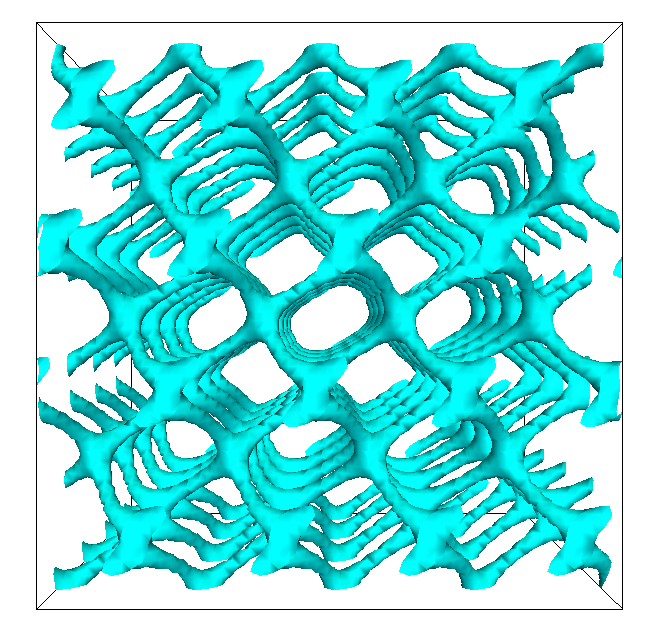
\includegraphics[width=0.35\textwidth]{disc-160k_run902.png}
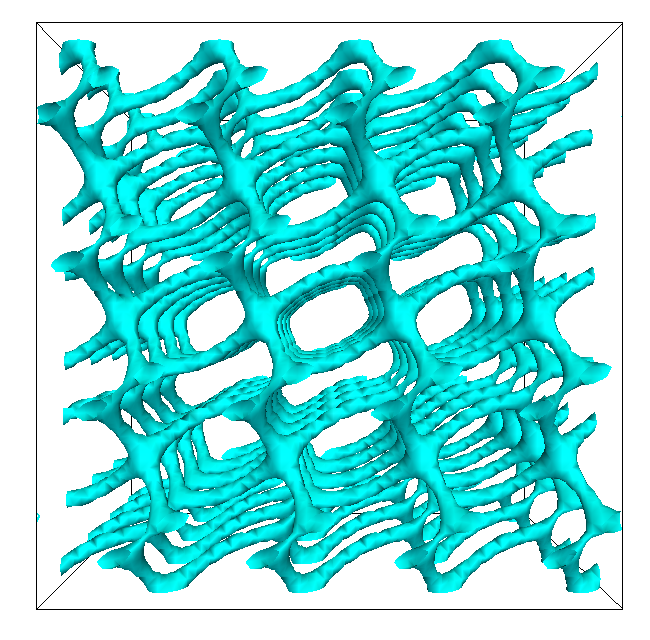
\includegraphics[width=0.35\textwidth]{disc-164k_run902.png}
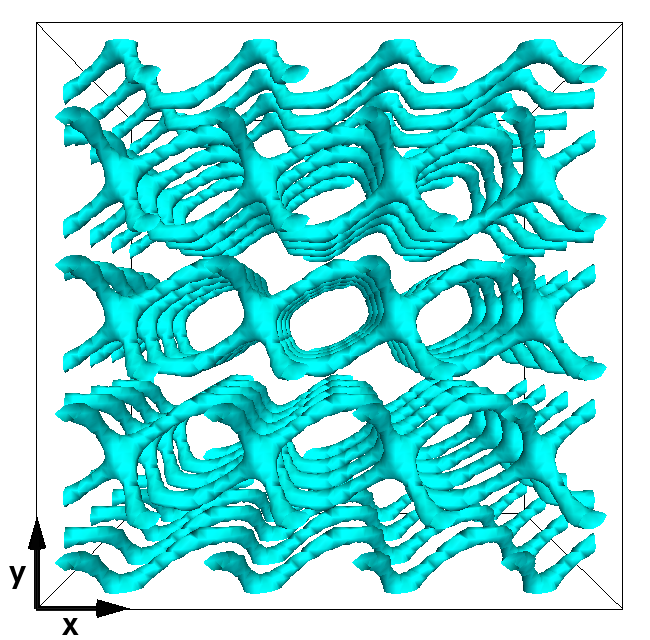
\includegraphics[width=0.35\textwidth]{disc-165k_run902.png}
\caption{Disclination network of BPII in shear flow: 
The pictures show a typical sequence of snapshots in the steady state 
at $\gd=1.56\e{-4}$ and time steps $t=1.60, 1.64,1.65\e{5}$. The velocity 
gradient is oriented along the vertical direction (y), whereas the 
horizontal direction (x) is the flow direction. Lees-Edwards boundary 
conditions have been imposed in such a way that the network moves to the 
right in the upper half and to the left in the lower half of the picture.}
\label{bp2-med}
\end{figure}

\begin{figure*}[htpb]
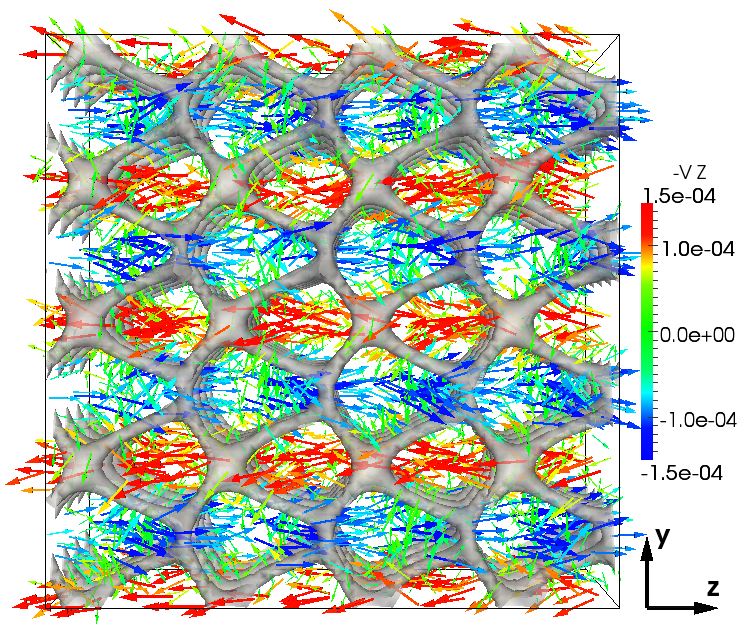
\includegraphics[width=0.495\textwidth]{v_yz-v_z-160k_run902.png}
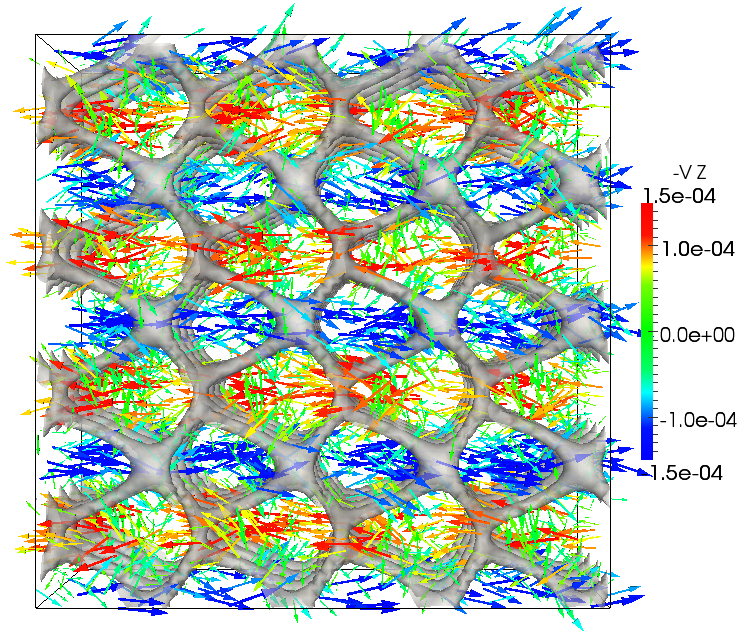
\includegraphics[width=0.495\textwidth]{v_yz-v_z-160k_run903.png}
\caption{Velocity patterns and disclination network in BPII for positive (left) and negative (right) helicity of the 
underlying cholesteric helix: The pictures show velocity vectors $(0,v_y,v_z)$.
The view is along the x-direction. This means the velocity ${\mathbf v}$ 
has been projected onto a plane perpendicular to the flow direction. 
The vertical and horizontal direction are the gradient and vorticity direction, respectively.
The colour code gives the magnitude and sign of the component in vorticity direction.
The snapshot shows a typical frame during a periodically recurring sequence.
The network on the left with right-handed helicity ($q_0>0$ in Eq.~\ref{FE}) travels rightwards, whereas the one one the right,
with reversed helicity, moves leftward. 
The periodicity of the motion along the vorticity direction is six times longer than the time 
it takes the network to reconnect along the flow direction.}
\label{bp2-velo}
\end{figure*}

Characteristic bands are visible in Fig. \ref{bp2-velo}, which are 
oriented along the vorticity direction. The direction of the flow
in each of the bands depends on the helicity of the underlying cholesteric
liquid crystal (i.e. on the sign of $q_0$ in Eq.~\ref{FE}), and the velocity
patterns for left-handed and right-handed BPs are one the mirror image of
the other. 
Further quantitative evidence for a direct link between the sense of motion 
and the helicity can be gained by time-averaging over individual cycles.

Table \ref{tab1} in the Appendix 
gives minima, maxima, averages and standard deviations 
of the velocity components.
All values for the two runs with inverted helicity are identical apart 
from a change of sign in the $z$-components.
There is only a slight imbalance in magnitude 
between the maximum and minimum velocities 
along the $z$-direction. Therefore the averaged flow along the vorticity
direction, leading to network motion, is very small, and much smaller than
the local velocity flow. This suggests that the
flow of the network along the vorticity 
direction is permeative (i.e. the fluid moves but the network as a whole 
moves much less). 

\subsubsection{Regime BPII-2: high shear rates }

If the flow rate exceeds a certain critical value BPII does not undergo the 
homogeneous deformation described above and adopts another mode of flow. 
Fig. \ref{bp2-high} shows a sequence of cuts through the director 
field at high shear rate. The entire blue phase network has broken up 
into a simple cholesteric helix and flows as a travelling 
helical wave with the helical axis oriented along the vorticity direction.
The state is translationally invariant in the flow and gradient directions.
It is the preferred mode of flow of a standard cholesteric phase
in vorticity mode at low Ericksen numbers. This is followed by
the uncoiling transition to a nematic, flow-aligned state at even 
higher shear rates ~\cite{Rey:1996a, Rey:1996b}.

In our scenario the BP to cholesteric transition occurs for shear rates $\gd\simeq 4.68\e{-4}$, which
corresponds to Ericksen numbers of ${\it Er}\simeq4$, based on our
parameters for BPII ($K=0.02, \eta=0.666$, and $p_0/2=16$;
see Table \ref{tab1} in the Appendix).

\begin{figure}[htpb]
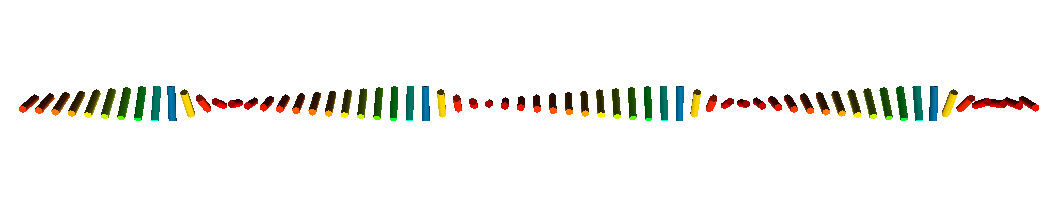
\includegraphics[width=0.495\textwidth]{dir+y-250k_run949.png}
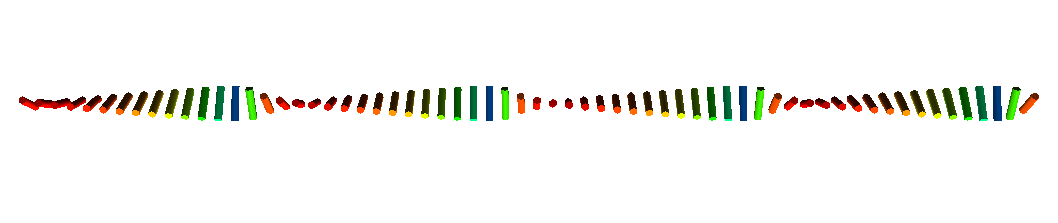
\includegraphics[width=0.495\textwidth]{dir+y-253k_run949.png}
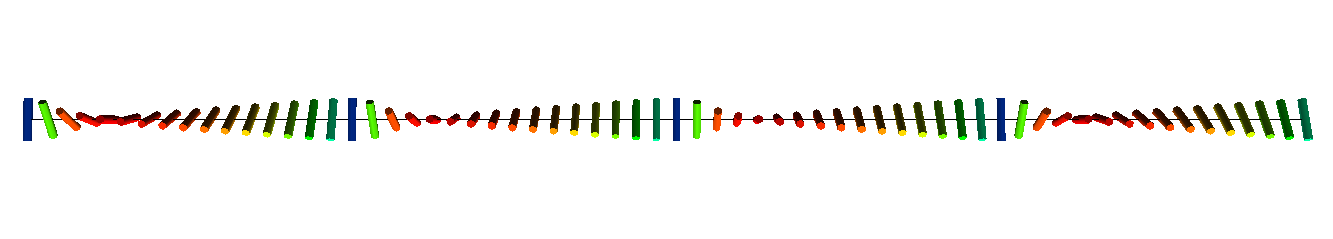
\includegraphics[width=0.495\textwidth]{dir+y-255k_run949.png}
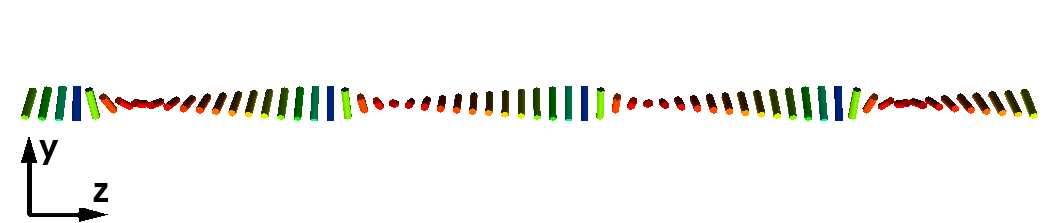
\includegraphics[width=0.495\textwidth]{dir+y-257k_run949.png}
\caption{Director field of BPII at high shear rate: The images show snapshots at time steps 
$t=2.50, 2.53,2.55, 2.57\e{5}$ (from top to bottom) with flow into/out of the page. The colour code gives the alignment of the director field in the flow direction (x) with red fully aligned and blue out of plane. 
The configuration is a helical wave that travels along the direction of vorticity.
It is translationally invariant along the gradient and flow direction.}
\label{bp2-high}
\end{figure}

We observe another configuration, lying between the travelling helical wave 
and the  flow-aligned nematic state at shear rates 
$7.81\e{-4}\lesssim\gd\lesssim9.37\e{-4}$ ($6.66\lesssim {\it Er} \lesssim 8$). In this interval
the helical axis now lies along the flow gradient direction (the so-called
Grandjean texture~\cite{deGennes}).
We will address this regime in section \ref{cholflow}, as it is common to BPI and BPII.

\subsection{Blue Phase I}

BPI has body-centred cubic symmetry and, unlike BPII, the disclination lines
characterising its equilibrium structure are well separated and do not 
intersect. (The quiescent state resembles the first frame in Fig.~\ref{bp1-low}
below.)
We believe that this topological difference is responsible for most of
the differences between BPI and BPII regarding their rheological response. 
We present again key aspects in an overview before we address specific features 
in more detail. 

Fig. \ref{bp1-rheo} shows the ratio between the 
apparent viscosity $\eta_{app}$ and $\eta$ versus time and 
strain for the same shear rates as in Fig. \ref{bp2-rheo}. The plot
shows that there is more shear thinning in BPI than in BPII, for
the shear rate range we considered. 
Through much of the flow range we studied,
the average shear stress versus shear rate can be fitted reasonably 
well by a power law $\bar{\Pi}_{xy}=a \gd^b$ with $a=0.019, b=0.63$.

For intermediate (but not low) shear rates, we once more find regular oscillations in the stress
response versus time, and in the network morphology -- we label this 
regime BPI-2. 
The BPI-2 regime now does not persist to arbitrarily low shear: there the
oscillations become irregular and seemingly chaotic, and after a few
cycles the disclination pattern becomes amorphous. We refer to this 
flow regime as BPI-1. 
The BPI-2 regime is also unstable if the shear is increased {\em above} 
a critical value -- close to this breakup point the oscillations in the 
shear stress show an increasingly complex
pattern, until the network breaks up completely and a new regime, BPI-3, is entered.
In regime BPI-3 ($6.25\e{-4}\lesssim\gd\lesssim7.81\e{-4}$; $10.67 \lesssim {\it Er} \lesssim 13.33$) 
we observe that the BPI network transforms under shear into
a  quasi two-dimensional state consisting of
double-twist rolls.
Finally, for shear rates such that
$9.37\e{-4}\lesssim\gd\lesssim1.25\e{-3}$ ($16 \lesssim {\it Er} \lesssim 21.33$) we observe the same cholesteric 
configuration with the helical axis along the gradient direction as 
reported above for BPII-2 (see
section \ref{cholflow}).
 

\begin{figure}[htpb]
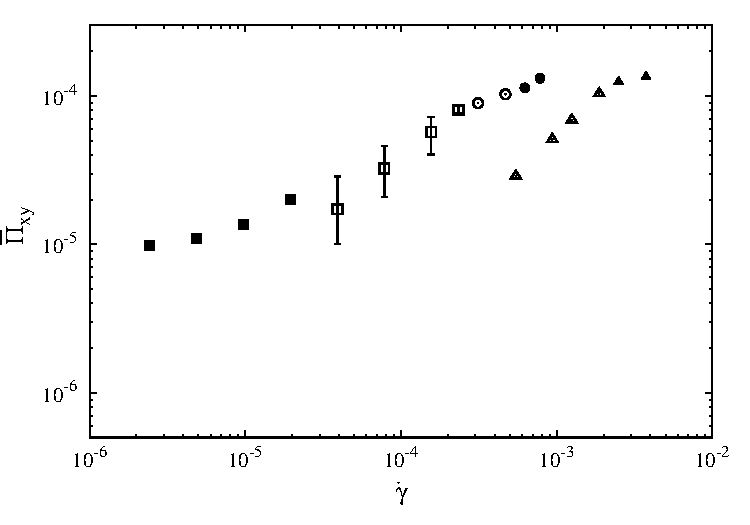
\includegraphics[width=0.495\textwidth]{flowcurve_bp1.pdf}\\
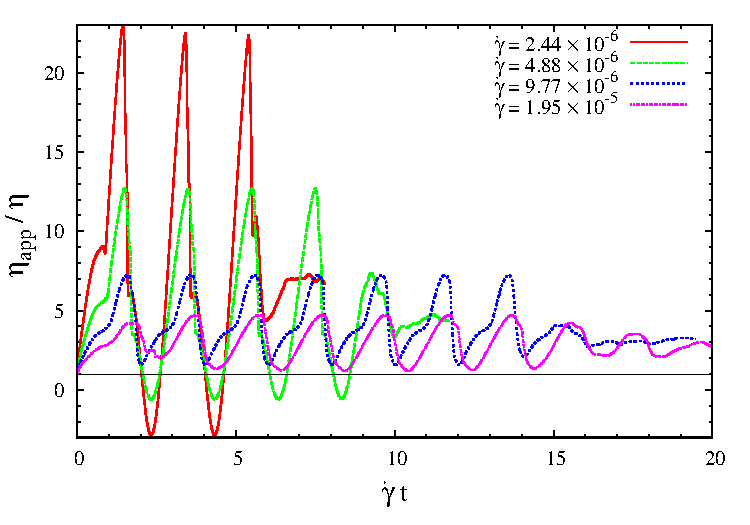
\includegraphics[width=0.495\textwidth]{app_visc_strain_bp1_a.pdf}\\
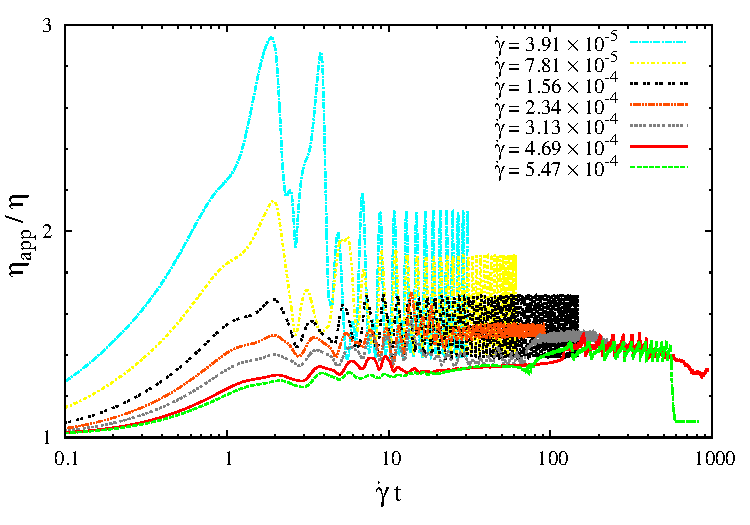
\includegraphics[width=0.495\textwidth]{app_visc_strain_bp1_b.pdf}\\
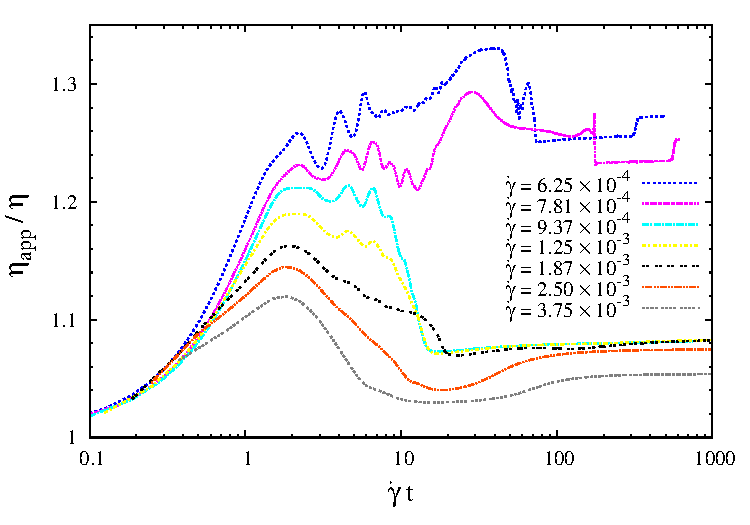
\includegraphics[width=0.495\textwidth]{app_visc_strain_bp1_c.pdf}
\caption{Apparent viscosity $\eta_{app}=\langle \Pi_{xy}\rangle/\dot{\gamma}$ (normalised by $\eta$) of BPI versus time (top) 
and strain (bottom). The inset shows the flow curve $\bar{\Pi}_{xy}(\gd)$. 
Depending on the configuration in steady shear flow three different regimes 
can be identified: amorphous BP network with yield stress (BPI-1, triangles), 
steady flow with recurring patterns (BPI-2, open circles), 
breakup of the disclination network (BPI-3, solid circle), 
cholesteric helix with axis in gradient direction (CHG, open squares) 
and flow-aligned nematic state (FAN, solid square). 
The error bars represent the minimum and maximum shear stress 
during one cycle. For clarity the individual curves have been shifted along
the time and strain axis.}
\label{bp1-rheo}
\end{figure}


\subsubsection{Regime BPI-1: low shear rates }

\begin{figure}[htpb]
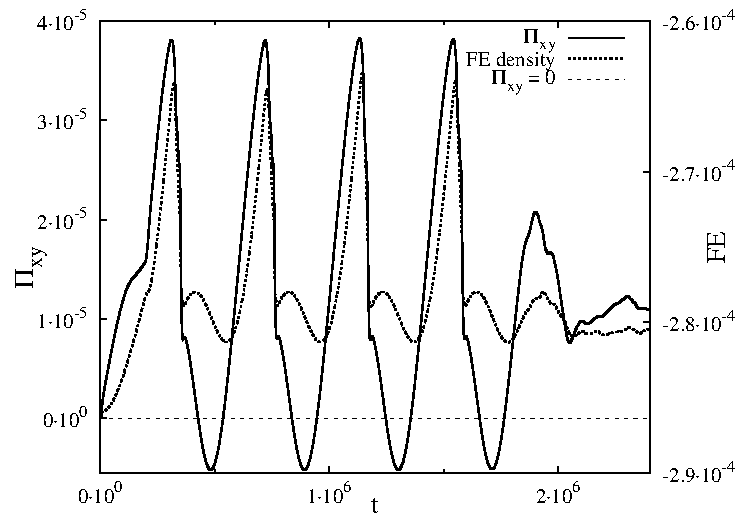
\includegraphics[width=0.495\textwidth]{stress_fe_yield_bp1.pdf}
\caption{Average thermodynamic shear stress and free energy density of BPI at shear rate 
$\gd=4.88\e{-5}, Er=0.08$: The negative branch in the stress is related to a local maximum and a following local 
minimum in average free energy density. This creates unstable conditions that lead 
to reconstruction of the defect lattice into an amorphous network state which 
seemingly features a yield stress.}
\label{bp1-fe-yield}
\end{figure}



The rheological response of BPI at low shear rate, $\gd\lesssim1.95\e{-5}$
(${\it Er} \lesssim 0.33$), 
is strikingly different from that of BPII and appears to show a
yield stress. An explanation for this behaviour can be found by 
looking more closely at the average shear stress (where the
background viscosity contribution has been subtracted) and 
free energy density as a function of time, as shown in Fig. \ref{bp1-fe-yield}.
When the quiescent and equilibrated BPI network begins to flow
the shear stress increases steeply and goes through a maximum.
Shortly after it goes negative (the total shear stress 
with the background viscosity contribution remains positive) 
to become positive again later on, forming a complete cycle.
The amplitude of the excursions in these stress oscillations, and
the presence of a part of the period where the thermodynamic
contribution to the stress is negative, suggest that the
BPI network is subject to large forces. Seemingly, these eventually
cause the flow-induced collapse to an amorphous network state with
an apparent yield stress. We should underscore that this
low shear regime might depend on our choice of boundary
conditions which in practice are equivalent to having infinitely
distant walls to which the network is anchored (see discussion
in the Appendix).
With free boundary conditions and for very low wall velocity, 
permeative flows might instead allow for
some slip of the BPI network, as in cholesterics sheared
along their axis~\cite{Marenduzzo:2006b}.

\begin{figure}[htpb]
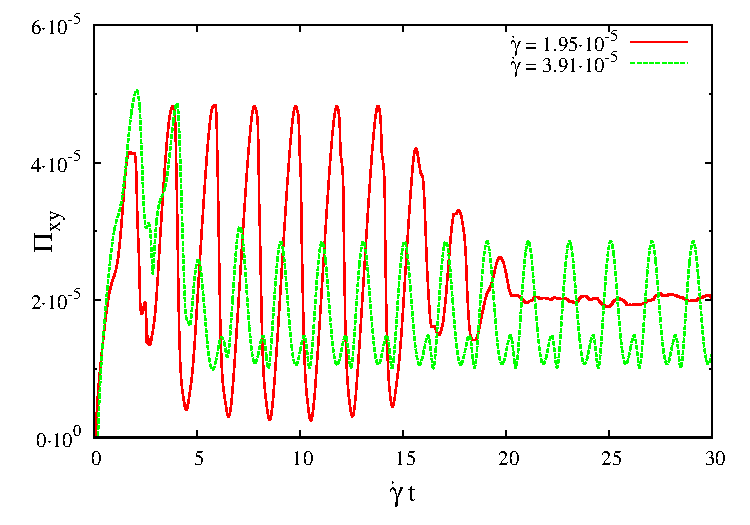
\includegraphics[width=0.495\textwidth]{stress_bp1-1_bp1-2.pdf}
\caption{Thermodynamic shear stress $\Pi_{xy}$ versus strain near the transition between regime
BPI-1 and BPI-2. The shear rates are $\gd=1.95\e{-5}$ (red solid) 
and $\gd=3.91\e{-5}$ (green dashed). Compared to lower shear rates in BPI-1 
where the stress goes negative (Fig. \ref{bp1-fe-yield}) the stress is 
throughout positive, but exhibits very large fluctuations during one cycle, 
which are absent in regime BPI-2 at higher shear rates than shown here.}
\label{bp1-1_bp1-2}
\end{figure}

\begin{figure*}[htpb]
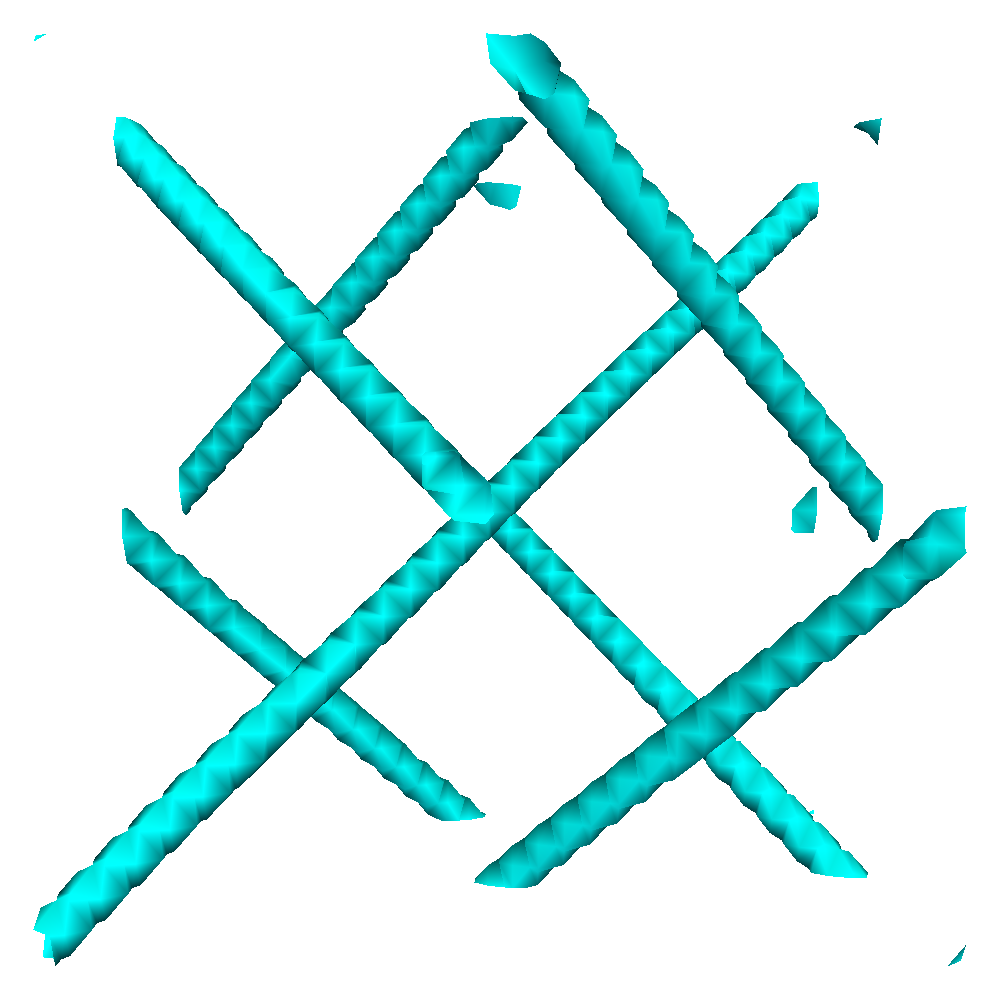
\includegraphics[width=0.245\textwidth]{disc-xy-10k_run1115.png}
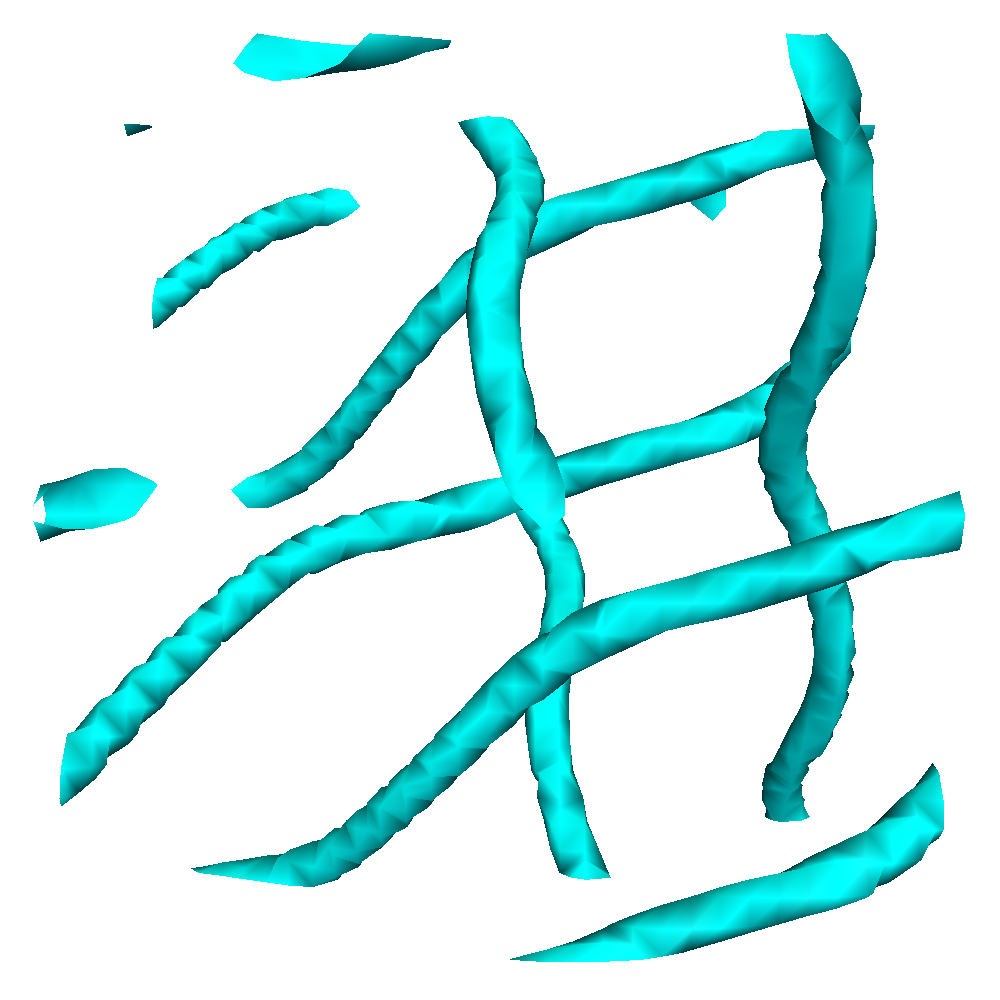
\includegraphics[width=0.245\textwidth]{disc-xy-180k_run1115.png}
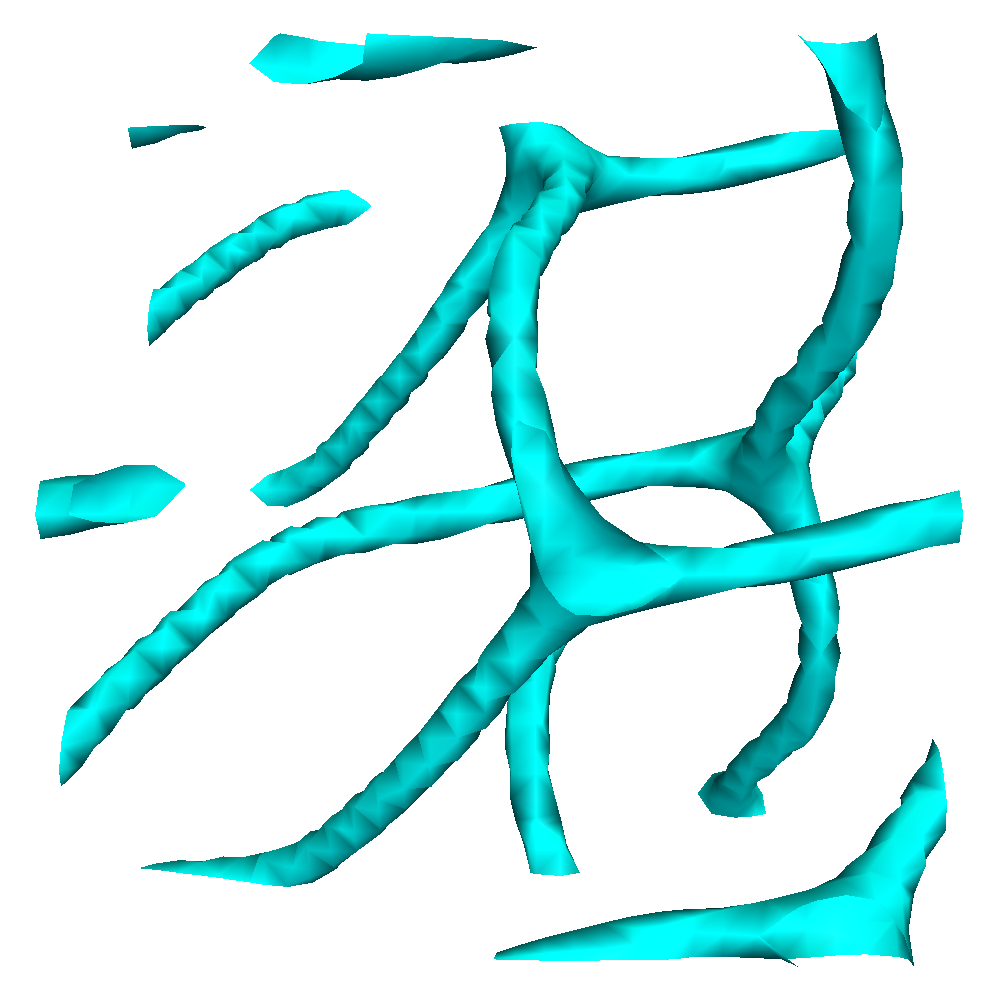
\includegraphics[width=0.245\textwidth]{disc-xy-200k_run1115.png}
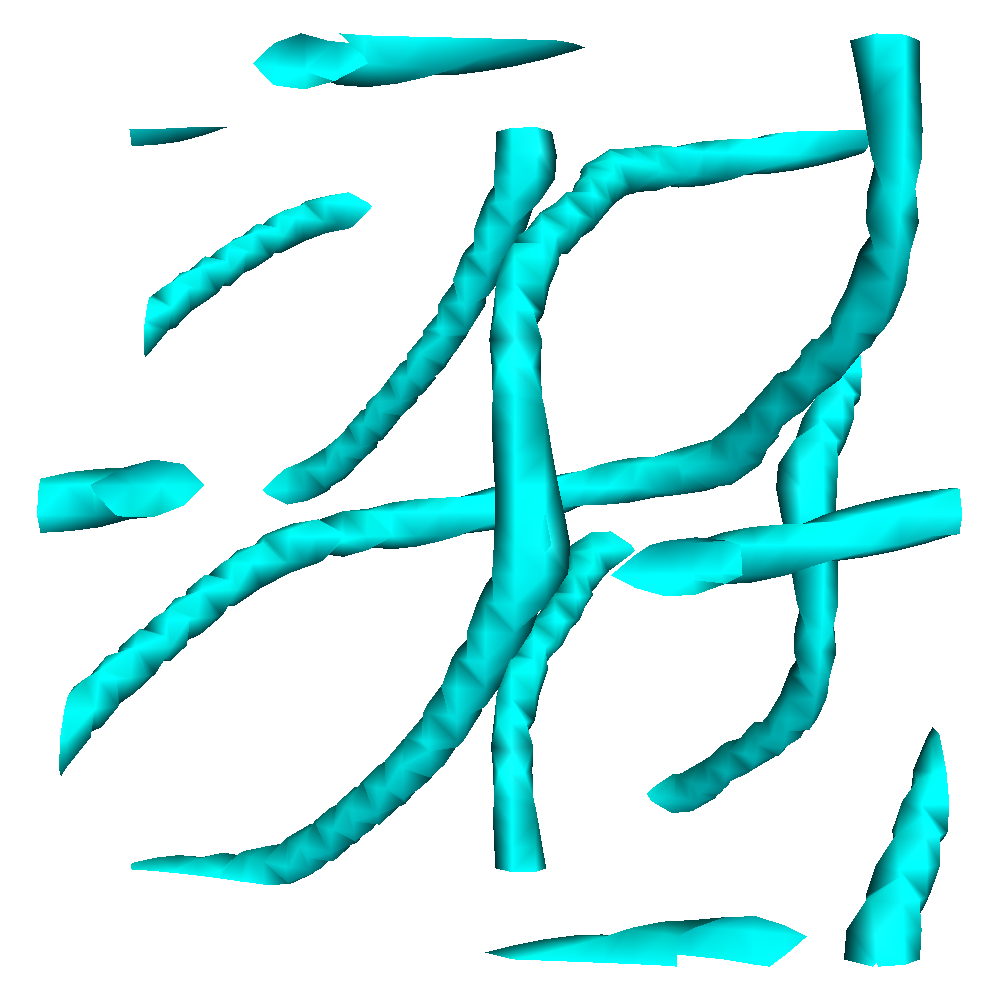
\includegraphics[width=0.245\textwidth]{disc-xy-210k_run1115.png}\\
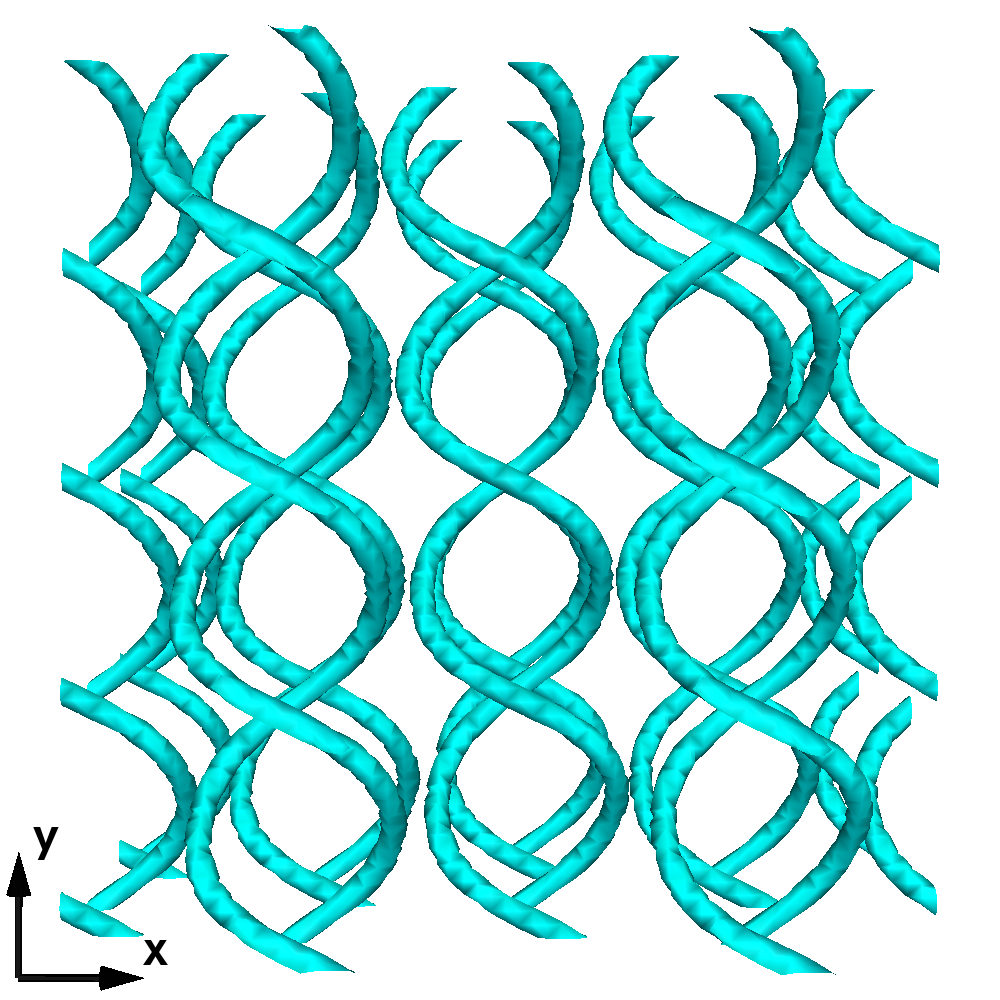
\includegraphics[width=0.245\textwidth]{disc-xy-400k_run1115.png}
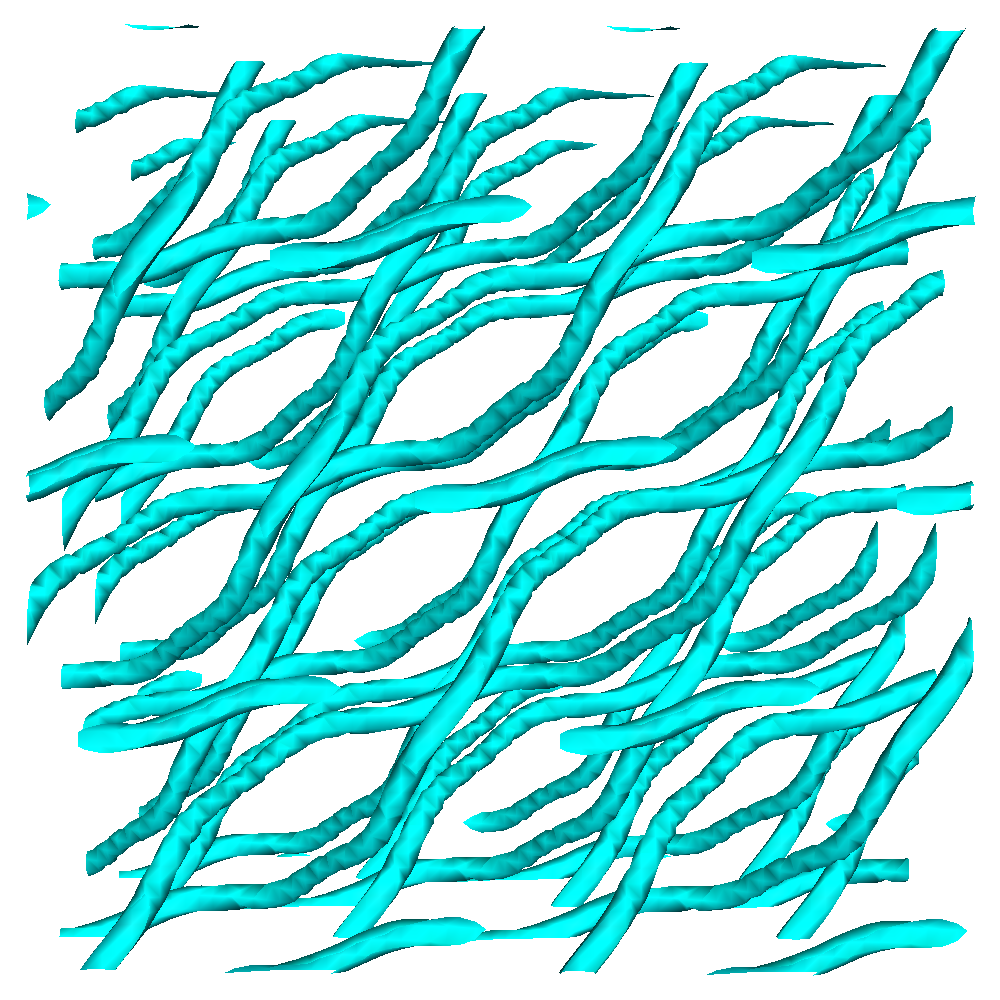
\includegraphics[width=0.245\textwidth]{disc-xy-700k_run1115.png}
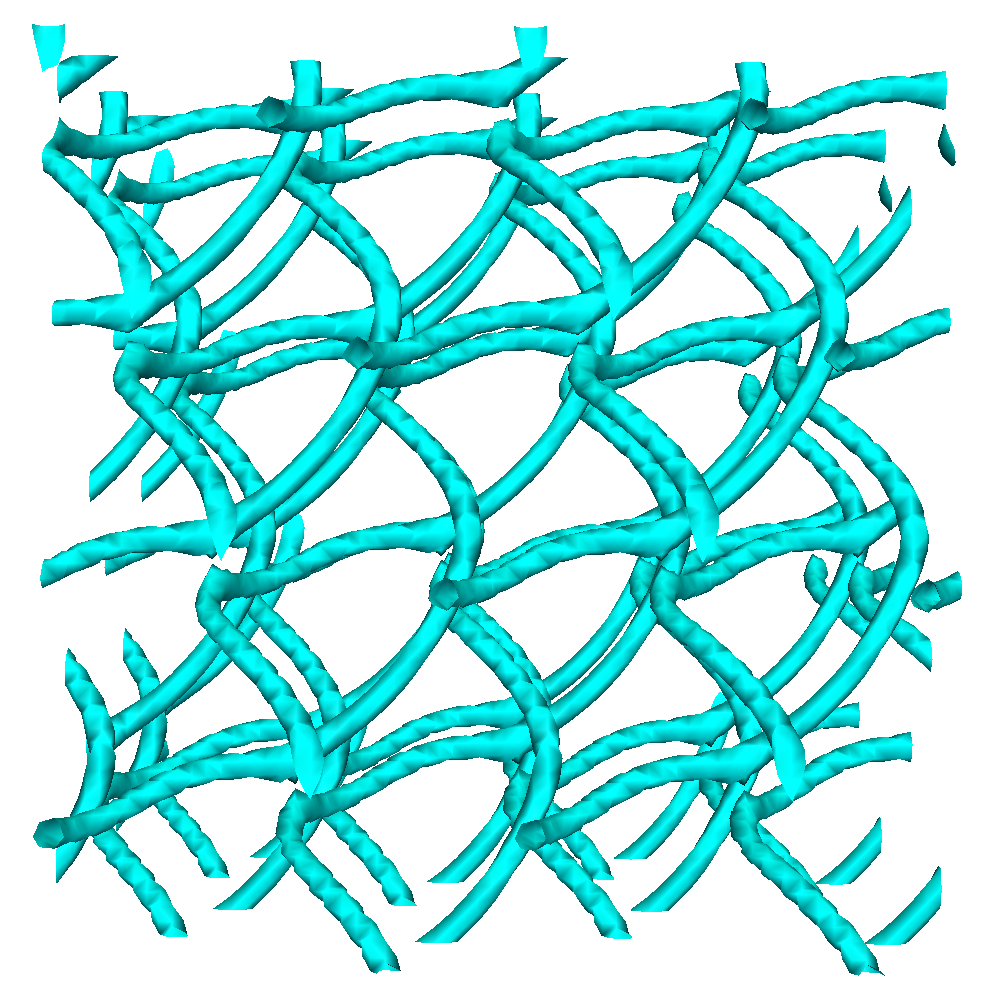
\includegraphics[width=0.245\textwidth]{disc-xy-750k_run1115.png}
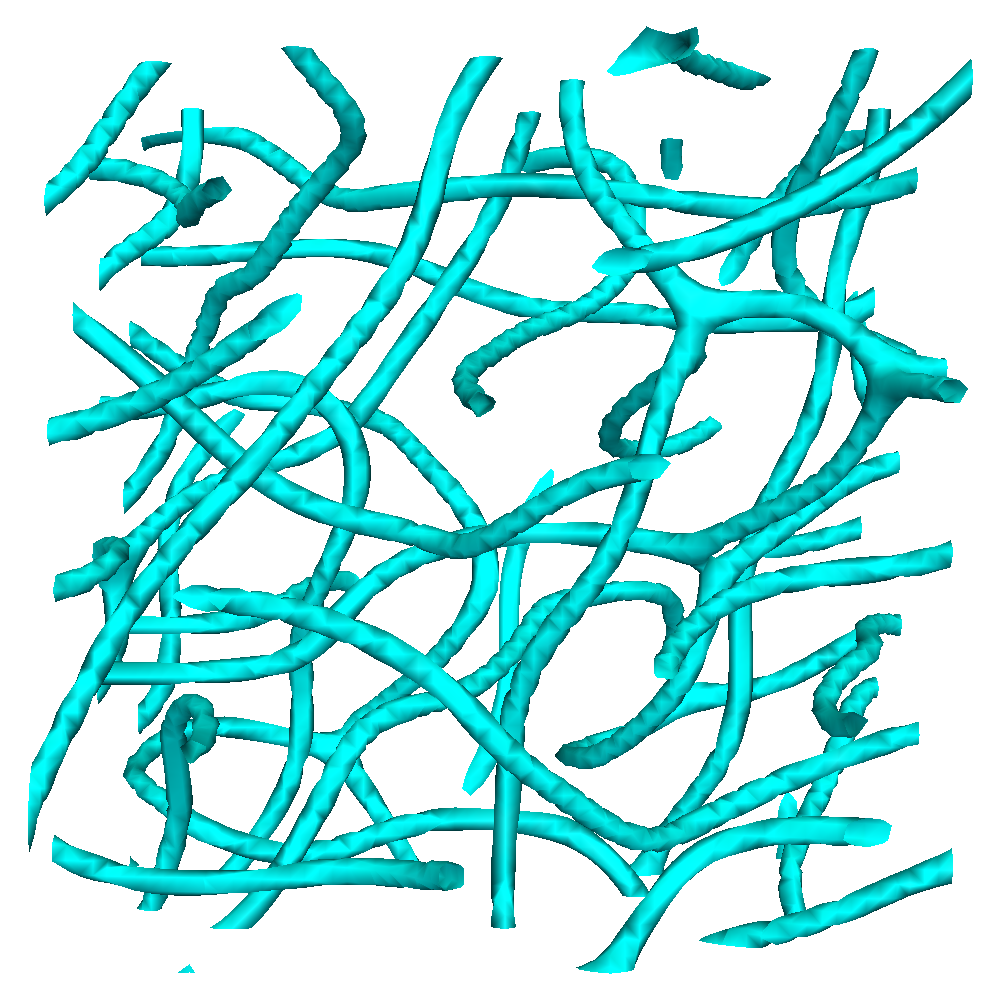
\includegraphics[width=0.245\textwidth]{disc-xy-2200k_run1115.png}
\caption{Snapshots of BPI disclination network at $\dot{\gamma}=4.88\e{-6}$: 
Depicted is the transition from the quiescent state to flow-induced, intertwined 
helices that undergo a recurring structural transformation. The top row
shows a section of one unit cell for early times 
$t=1\e{4}, 1.8\e{5}, 2.0\e{5}$ and $2.1\e{5}$. The bottom 
pictures on the far left, centre left and centre right 
show the situation at later time steps $t=4.0, 7.0$ and $7.5\e{5}$,
which the system passes for several cycles before it ends up in
an amorphous state (bottom row far right, at time step $t=2.2\e{6}$).}
\label{bp1-low}
\end{figure*}

\if{The negative branch in the shear stress is connected
to a local maximum followed by a local minimum in the 
average free energy. Hence, the region of negative stress can be 
regarded as a phase during which elastic forces exert a 
'pull' on the network while it tries to reach a more 
favourable configuration. However, the low flow rate
causes this unstable intermediate state to be exposed to these
elastic forces for a relatively long time, long enough to 
create small distortions which finally break the symmetry of the
flow-induced configuration.}\fi


To gain further insight into the flow-induced deformation, and eventual
breakdown, of BPI, it is instructive to follow the dynamics of 
the network under a slow flow -- this is depicted in Fig. \ref{bp1-low}.
Three different stages can be distinguished. 
Just after the onset of the shear flow, the disclination lines 
in BPI get more and more squeezed together, and this is incompatible with
the defect topology in this phase.
Consequently, the network adopts a flow-induced conformation which consists 
of intertwined helices that stretch during the shear transformation.
This helical conformation that emerges already at strains $\gamma\simeq1$ 
is shown in Fig. \ref{bp1-low} (top row).
At this point the original BPI has already been significantly deformed.
Shortly afterwards regular oscillations set up temporarily,
where the disclinations form double helices which tilt and realign under the shear.
There is no perceivable movement of the 
network along the vorticity direction at any stage of the cycle.
(This contrasts with the BPII-2 results reported earlier.)

This mode of flow proves unstable, as after a few cycles 
distortions appear which lead to further destabilisation -- presumably in
view of the large stress fluctuations discussed above. 
Finally, the system loses order and 
transforms into an amorphous network state with almost constant
stress in the region of $\Pi_{xy}\simeq 1\e{-5}$ LBU.
If the shear is stopped, this flow-induced amorphous state
remains arrested and metastable, and cannot
find its way back to the original BPI structure.

\subsubsection{Regime BPI-2: intermediate shear rates }

Adjacent to regime BPI-1 ($\gd\lesssim1.95\e{-5}$; $ {\it Er}\lesssim 0.33$) but 
at slightly larger shear rates ($3.91\e{-5}\lesssim\gd\lesssim 4.687\e{-4}$; $0.67\lesssim{\it Er}\lesssim8$)
lies another region where the network flows with periodically 
recurring conformations (Fig. \ref{bp1-rheo}). 
We refer to this region as BPI-2. The transition between BPI-1 and BPI-2 
is clear when looking at Fig. \ref{bp1-1_bp1-2} 
which shows the shear stress versus total strain. 
A qualitative difference between these two is the absence in BPI-2 of the 
large stress fluctuations that occur during the early cycles in regime BPI-1.
(Recall that for even lower $\gd$ the thermodynamic shear stress becomes 
temporarily negative (Fig. \ref{bp1-fe-yield}), which 
caused destabilisation of the periodic network and led to the 
amorphous configuration in the steady state.)
Hence, an explanation
for the existence of the regular BPI-2 oscillations 
could be that these are fast enough to bypass or suppress 
large stress fluctuations -- this leads to
a different order structure and to a stabilisation 
compared to the oscillations found transiently in
the BPI-1 regime.

\begin{figure*}[htpb]
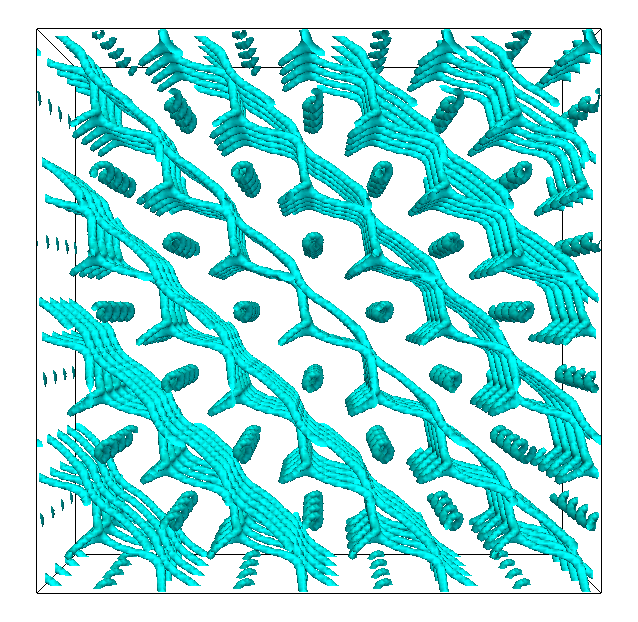
\includegraphics[width=0.32\textwidth]{disc-365k_run914.png}
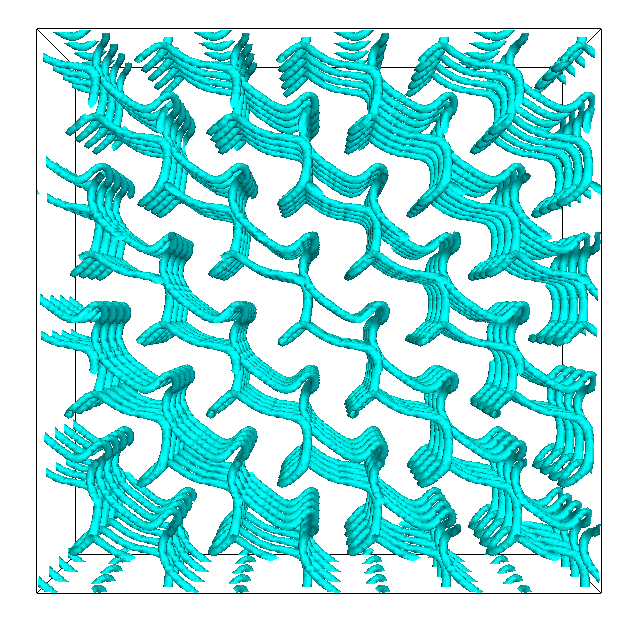
\includegraphics[width=0.32\textwidth]{disc-367k_run914.png}
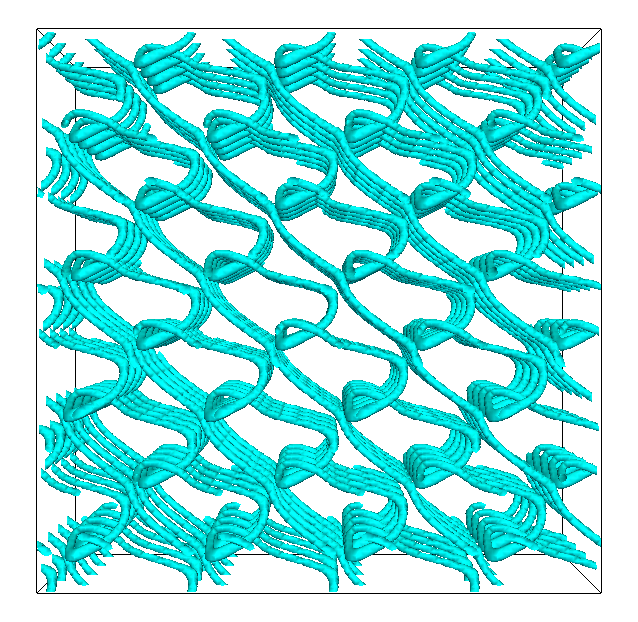
\includegraphics[width=0.32\textwidth]{disc-375k_run914.png}\\
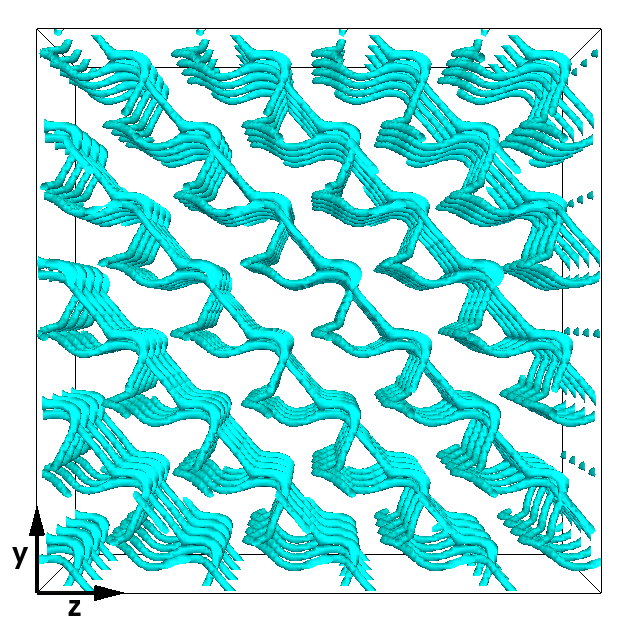
\includegraphics[width=0.32\textwidth]{disc-380k_run914.png}
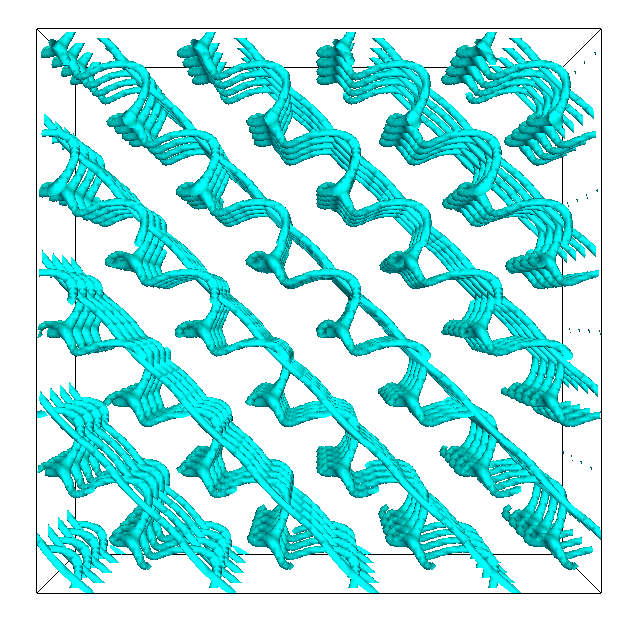
\includegraphics[width=0.32\textwidth]{disc-384k_run914.png}
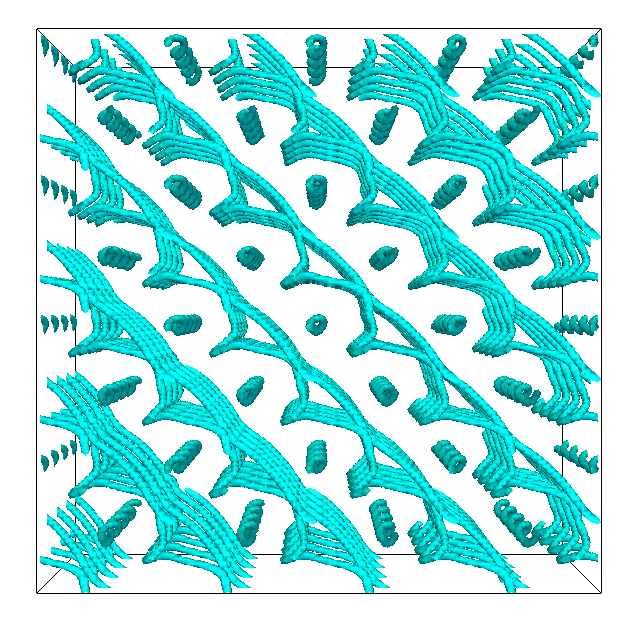
\includegraphics[width=0.32\textwidth]{disc-389k_run914.png}
\caption{Disclination network of BPI in regime BPI-2 (intermediate flow rates): 
The sequence shows a typical cycle of shear-induced transformations in the 
steady state at $\gd=1.56\e{-4}$ and time steps 
$t=3.65, 3.67,3.75,3.80,3.84,3.89\e{5}$ with the flow into/out of the page. 
During every cycle the network is displaced also along the gradient and vorticity direction, 
but the magnitude and direction of the offset does not appear to obey a 
simple rule.}
\label{bp1-med}
\end{figure*}

\begin{figure*}[htpb]
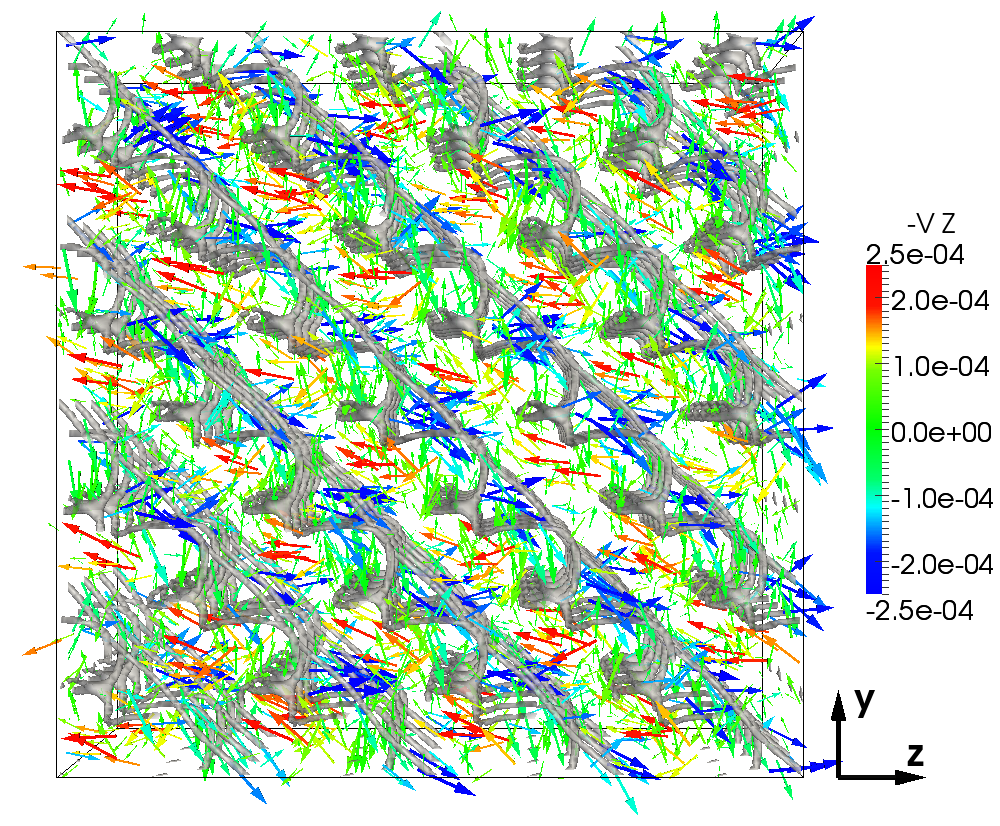
\includegraphics[width=0.495\textwidth]{v_yz-v_z-360k_run914.png}
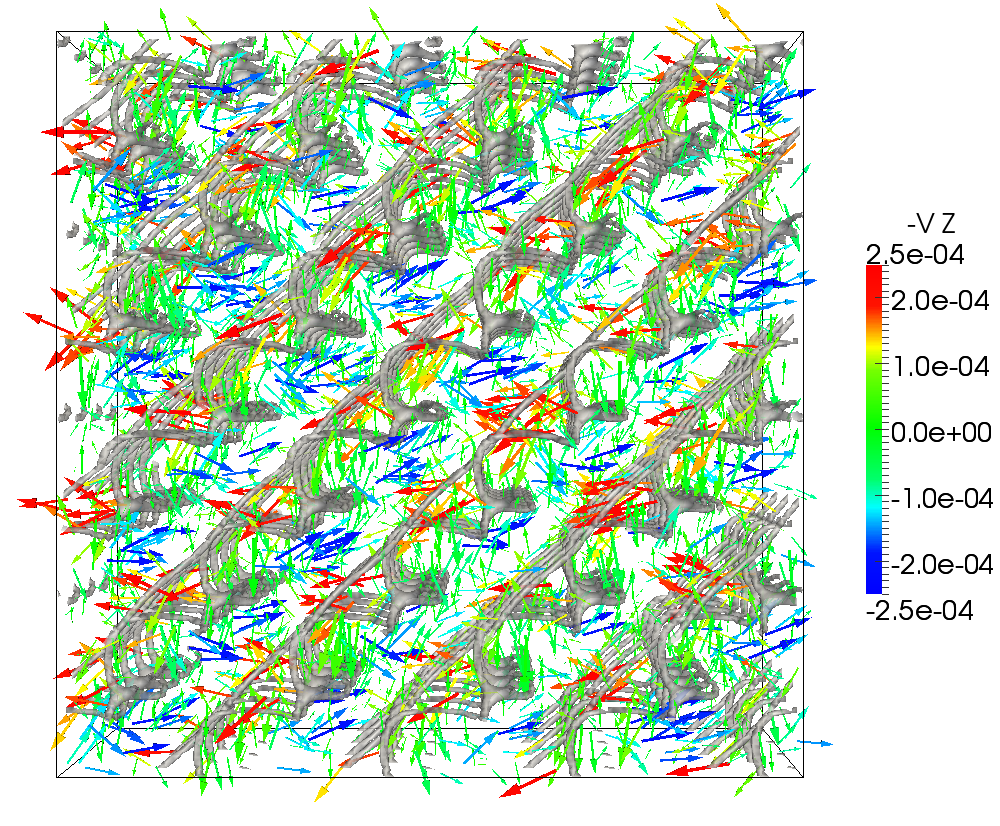
\includegraphics[width=0.495\textwidth]{v_yz-v_z-360k_run922.png}
\caption{Velocity patterns in BPI for positive (left) and negative (right) helicity: 
The pictures show a snapshot of the periodically recurring patterns in the 
secondary velocity components $(v_y,v_z)$. 
The colour code gives the magnitude and sign 
of the $z$-component. The vertical and horizontal direction are the gradient and 
vorticity direction, respectively, with the flow into/out of the plane in the 
upper/lower half of the images.}
\label{bp1-velo}
\end{figure*}

Fig. \ref{bp1-med} shows snapshots of the periodically recurring 
BPI in steady shear flow. Contrary to BPII-1 at these shear rates, 
BPI-2 does not resemble the equilibrium configuration
undergoing a homogeneous topology-conserving 
transformation. It features rather intricate, flow-induced 
conformations. Surprisingly, if the shear is switched off in
the BPI-2 regime at some point during an oscillation, 
the flow-induced configuration usually
reverts to a perfect quiescent BPI -- in stark contrast with
what happens in BPI-1, for lower shear rates. 

Finding the recurrence period for BPI is not simple, as
this depends subtly on the applied shear rate. The analysis is complex for
a number of reasons. 
First, the recurrence period for the stress is not always the same as
that of the network configuration. 
For instance, at $\gd=3.9062500\e{-5}$, it takes $2/\gd$ for one
 stress cycle to complete, but $4/\gd$ for the network to recur --
this is because the configurations at times $t$ and $t+2/\gd$ are 
mirror-images. This is by no means generic though: for example
at $\gd=4.8828125\e{-5}$  it takes $8/\gd$ for one
stress cycle to complete, but $16/\gd$ for the network to recur. 
For some higher shear rates, the recurrence period of stress
and network conformations are instead the same.
Second, there exist isolated values (or perhaps small ranges) of shear
rates for which the recurrence period is much longer and far more irregular,
with seemingly intermittent dynamics (e.g. at $\gd=1.3671875\e{-4}$ the
network configuration repeats itself after $6/\gd$, $12/\gd$, $22/\gd$).
Taken together, all this evidence very much suggests that 
the BPI-2 range includes at least some instances of ``rheochaos''~\cite{rheochaos,Cates:2002}.

Fig. \ref{bp1-velo} depicts a snapshot of the secondary velocity 
components $v_y$ and $v_z$ for left- and right-handed chirality of
the blue phase. The emerging pattern is similar to that of BPII from 
Fig. \ref{bp2-velo}, but differs in that there is no simple
separation into bands with opposite secondary velocity. 
However, just as in the case of BPII, both patterns
are mirror images and feature the highest velocities in the regions where 
the largest conformational changes take place. 

\if{In order to gain a better understanding of the complex oscillatory behaviour in regime BPI-2 
we performed a Fourier analysis of the shear stress $\Pi_{xy}$ according to Eq. \ref{spectrum}. 
The spectrum is shown in Fig. \ref{bp1-spectrum}. 

There are two aspects which are worth mentioning. First, we observe a strong contribution of 
the fundamental mode for the lowest two shear rates and a relatively small contribution of higher harmonics. 
However, at $\gd=1.563\e{-4}$ and $3.125\e{-4}$ the relative contribution of higher harmonics is 
significantly larger. 
Second, more surprisingly, the frequency of the fundamental mode is the same 
for all three shear rates $\gd=7.81\e{-5}, 1.563\e{-4}$ and $3.125\e{-4}$. This is 
in contrast to what is observed at lower flow rates. By doubling the flow rate from 
$\gd=3.91\e{-5}$ to $\gd=7.81\e{-5}$ the peak position in the spectrum 
moves to double the frequency. This means that the fundamental mode at flow rate $\gd=7.81\e{-5}$ 
coincides with the the first harmonic at $\gd=3.91\e{-5}$, the first harmonic with the third and so on. 
At higher shear rates in regime BPI-3 this 'lock-in' of flow modes disappears again.  
 
Interestingly the lock-in has only a minor effect on the flow velocities themselves.
The average velocities in Tab. \ref{tab1} (see Appendix) reveal that only the magnitude of some of the secondary 
flow components $v_y$ and $v_z$ appears to be relatively small compared to the primary component $v_x$. 
The latter is directly linked to the imposed shear rate. }\fi

\if{
\begin{figure}[htpb]
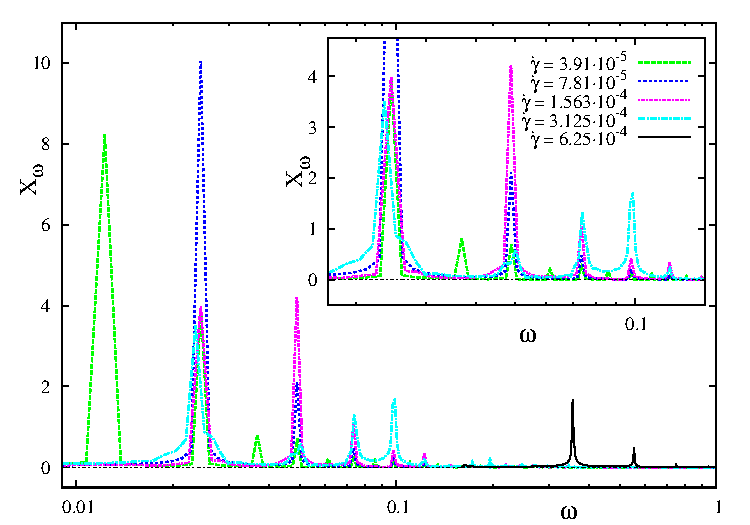
\includegraphics[width=0.495\textwidth]{spectrum_bp1.pdf}
\caption{Fourier analysis of the shear stress $\Pi_{xy}$ of BPI: The main picture shows 
spectral components and the 'lock-in' of flow modes, 
visible in the fixed peak position for certain flow rates.  
The inset shows a zoom of the same data over 
a portion of the frequency range.
The frequency is given in inverse time, in simulation units. TRUE?
OH: I WOULD SAY NO AS IT IS IN UNITS OF 2$\pi$ (RADIANS?).}
\label{bp1-spectrum}
\end{figure}
}\fi 

The intricacy and periodic recurrence of the flow-induced conformations 
in BPI raises the question: how robust are these results to variations in 
system size? Although a pitch length of 64 LBU provides enough resolution 
for tracking the network in flow it is not clear whether $4^3=64$ unit cells 
in total are actually sufficient to avoid finite size effects.
Unfortunately the computational costs of larger simulations are still
quite prohibitive (in the region of ${\it O}(10^5)$ core hours per run at
doubled system size), given that large strains have to
be simulated in order to reach a steady state. Therefore we opted for a 
comparison with smaller runs.

\begin{figure}[htpb]
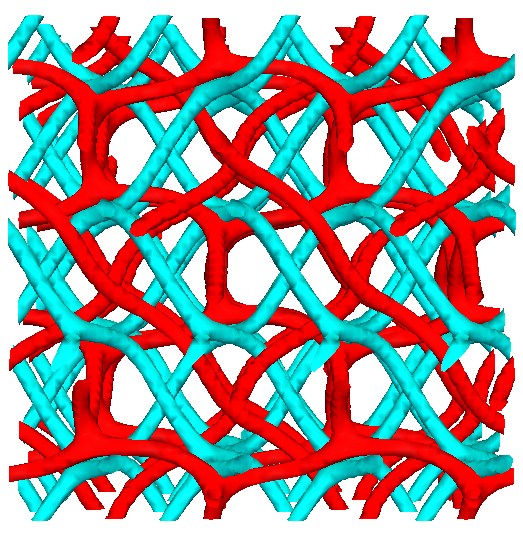
\includegraphics[width=0.43\textwidth]{disc+y-600k-run911_run1163.png}\\
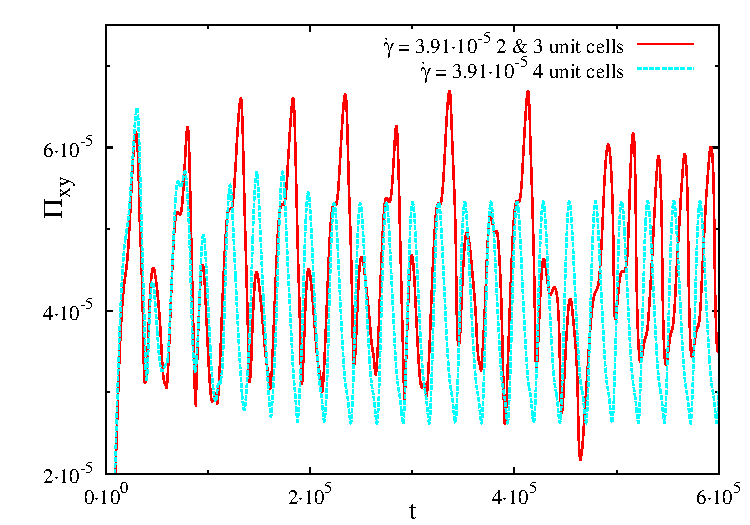
\includegraphics[width=0.495\textwidth]{stress_bp1_2uc_4uc.pdf}
\caption{Disclination network and shear stress $\Pi_{xy}$ in BPI: 
The dark (red) network in top picture shows a snapshot of run that consists 
of $2^3=8$ unit cells, whereas the light (cyan) network displays the 
central section of 8 unit cells in a bigger run with $4^3=64$ unit cells altogether. 
The bottom picture shows the shear stress over time. (Interestingly, 
an intermediate sized run with $3^3=27$ unit cells led to results that 
were virtually identical to the smaller run with 8 unit cells.) 
The shear rate was $\gd=7.81\e{-5}$.
}
\label{bp1-2uc4uc}
\end{figure}
 
Fig. \ref{bp1-2uc4uc} shows a comparison of the disclination network and 
shear stress $\Pi_{xy}$ of two different runs, one consisting of 8 
unit cells and the other one with 64 unit cells.
We observe that there are deviations in the visual appearance of the 
network as well as in the time-dependence of the shear stress.
Perhaps surprisingly, the smaller run with 8 unit cells takes longer 
to reach the steady state with its flow-induced recurring disclination network. 
These results indicate that we cannot know with certainty whether the individual 
flow-induced conformations that we find for 64 unit cells are affected 
by the imposed periodicity -- quite possibly the details of the oscillations
would differ in an even larger simulation. 
Nevertheless, the comparison suggests that 
the recurrence period and the complexity of the network in flow are  
generic features of BPI in this regime of flow.

\subsubsection{Regime BPI-3: high shear rates }

At high flow rates, $6.25\e{-4}\lesssim\gd\lesssim7.81\e{-4}$ ($10.67\lesssim {\it Er}\lesssim 13.33$), 
we observe a break-up of the flow-induced 
disclination network of regime BPI-2. However, 
in contrast to BPII, where the configuration is a travelling helical 
wave (cf. Fig. \ref{bp2-high}), BPI breaks down into a quasi 
two-dimensional, translationally invariant state, which is shown in 
Fig. \ref{bp1-high}. 
There are distinctive regions where the director field is 
predominantly oriented along the vorticity direction and 
other regions where it is oriented rather in flow-gradient plane. 
Occasionally, while moving past each other, these rolls resemble 
regions of local double twist.
Interestingly the critical Ericksen number for the break-up lies in 
about the same window as that of transition between BPII-1 and BPII-2. 

\begin{figure}[htpb]
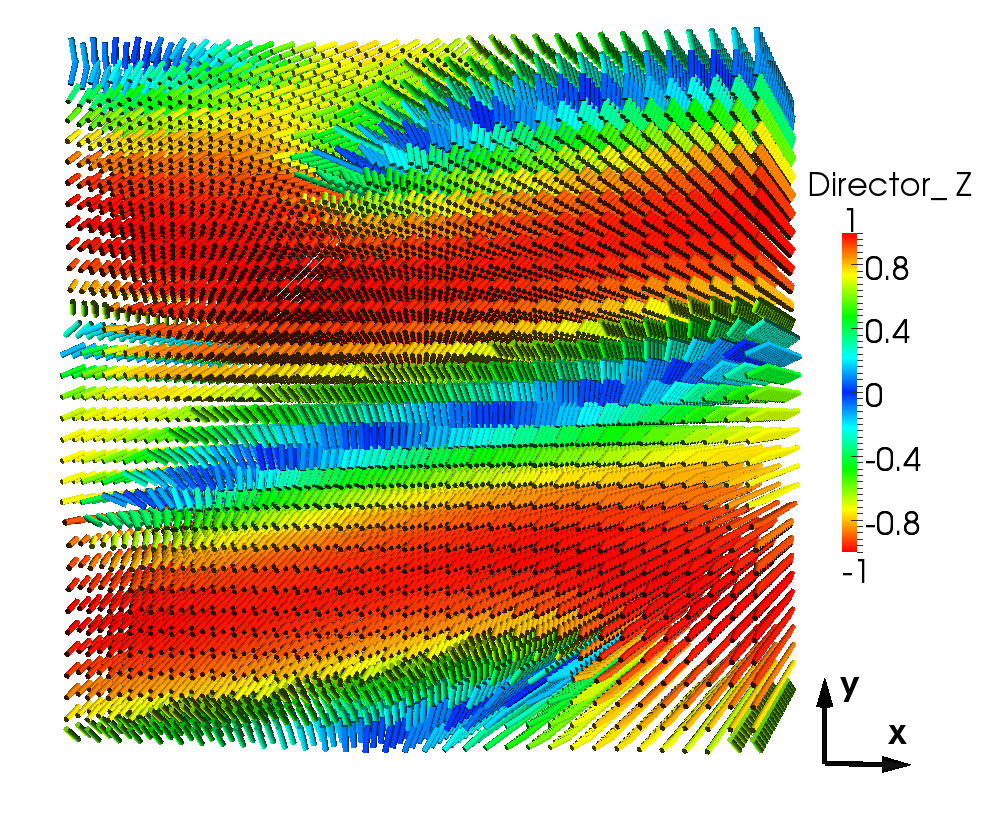
\includegraphics[width=0.45\textwidth]{dir3d-z-302k_run916.png}
\caption{Director field of BPI at high shear rate: The pictures show a region 
of $L_x\times L_y \times L_z= 32^3$ lattice sites with the flow/gradient 
direction oriented along the horizontal/vertical axis. 
The colour code gives the magnitude of the z-component of the director field. 
The data show that the structure is quasi-2D, with rolling double twist
patterns in the $xy$ plane, and an approximate translational symmetry 
along the vorticity direction.}
\label{bp1-high}
\end{figure}

\subsection{Transition to cholesteric helix and flow-aligned nematic state}\label{cholflow}

At shear rates beyond the regimes BPI-3 and BPII-2, but below the transition to a 
flow-aligned nematic state at still higher shear rates, we found another regime where 
both blue phases adopt the same configuration in steady shear flow, 
independent of their initial state.
The director field of this configuration is shown in Fig. \ref{fig:cholflow}.
It consists of a simple cholesteric helix with the helical axis oriented 
along the velocity gradient direction. The state is translational invariant 
along the flow and vorticity direction and therefore also one-dimensional. 
However, in contrast to the travelling helical wave of BPII-2 the 
director field is now static and there is no tumbling motion. 
While flowing the director retains its relative orientation.
Consequently, the shear stress is lower than for
the 2D double-twist rolls of BPI-3 and the travelling helical wave
(Fig. \ref{bp2-rheo} and \ref{bp1-rheo}) as there is less dissipation.
 
\begin{figure}[htpb]
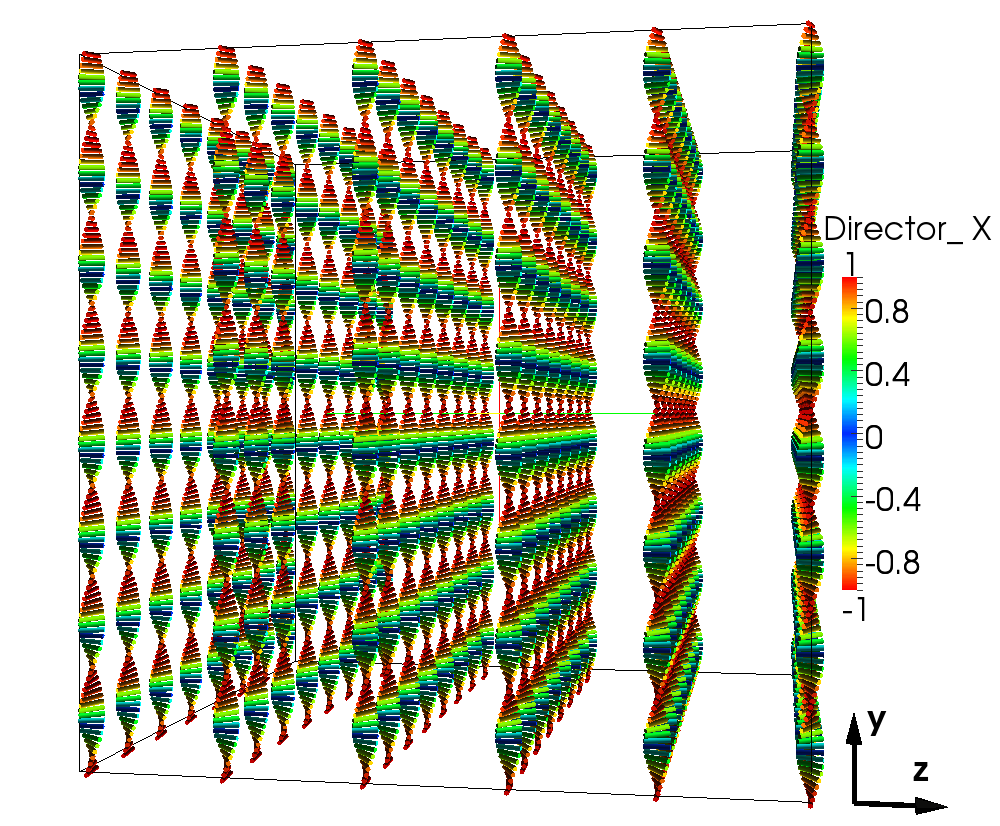
\includegraphics[width=0.45\textwidth]{dir3d+y-200k_run1179.png}
\caption{Flow induced cholesteric state. The orientation of the helix is 
along the gradient direction. The director field is quasi-static during 
the flow, which occurs in ``nematic layers''. Colour coding indicates the 
$x$ component of the director field (see colorbar on the right).
For clarity only selected sites are shown along the $y$-direction (along which
the structure is translationally invariant).}
\label{fig:cholflow}
\end{figure}



%\clearpage

\section{Conclusions}

In summary, our work constitutes the first large scale simulation of bulk flow behaviour 
of cubic BPs in simple shear flow. 
  
We were able to characterise the rheology of cubic BPs, and identified 
two different flow regimes for BPII and three different ones for BPI. 
Below an Ericksen number of $Er\simeq3$, BPII exhibits weak shear-thinning and 
obeys a power-law flow curve with exponent close to unity.  
The BPII disclination network breaks up and reconnects 
in the flow, which leads to a periodically recurring dependence 
of the shear stress. The flow-induced conformation looks generally
very similar to the quiescent network at equilibrium. 
While being homogeneously transformed due to the shear flow
the disclination network moves steadily in the vorticity direction
apparently by a permeation mechanism. The sense of
motion is directly linked to the helicity of the underlying cholesteric phase.

At larger Ericksen numbers, $4\lesssim Er\lesssim 10$, the flowing BPII network 
breaks up in a two-step manner. First a simple cholesteric helix forms with the helical axis 
along the vorticity direction. The flow excites a travelling helical wave,
as predicted theoretically in Ref.~\cite{Rey:1996a,Rey:1996b}.
Upon increasing the shear, the helix rotates and orients along the
gradient direction, where it can support larger flow rates due to the translational
symmetry along the flow direction. Still larger flow rates break this residual
cholesteric order and leave a standard flow-aligned nematic state,
at the highest shear rate studied.

Interestingly, BPI shows a flow behaviour that is very different to that of BPII.
This is a direct consequence of the topological differences between their disclination 
networks. Below an Ericksen number of $Er\sim 0.4$, the BPI network cannot both flow and 
retain a regular appearance. It eventually reorganises into an amorphous network that
features yield-stress behaviour. The apparent reason is that shortly after the onset of the shearing 
very large stress fluctuations occur. At the lowest shear rates
the thermodynamic contribution to the shear stress becomes temporarily 
negative during each cycle. These fluctuations seem to destabilise the network and 
eventually trigger the transition into an amorphous state with a residual yield
stress. 

At slightly larger Ericksen numbers $0.4\lesssim Er \lesssim8$,
BPI kinematically bypasses the large stress fluctuations and 
flows with very complex, periodically recurring flow-induced conformations.
These conformations entail regularly arrange helical disclinations which 
rotate due to the shear -- a new flow-induced state which was not previously
predicted. 
The oscillatory dynamics is in some cases intermittent, and the
recurrence period for the network conformations and stress patterns
is not given by a simple formula as for BPII.
Despite their complex appearance, the flow-induced conformations are 
topologically connected to the quiescent BPI and after switching off the 
shear flow a defect-free blue phase reforms. It is tempting to
interpret the unsteady oscillations seen in this regime as an instance of 
deterministic rheological chaos~\cite{fielding, Cates:2002}.

Just as in the case of BPII, the BPI network breaks up at larger Ericksen numbers in
a two-step process. First, at $10\lesssim\ Er\lesssim 15$, it adopts a 
quasi-two-dimensional configuration that is translationally invariant along vorticity direction. 
Then, at $16\lesssim Er \lesssim 22$, it forms a cholesteric helix along the flow gradient 
direction.  Finally, at $Er\gtrsim30$ (BPI) and $Er\gtrsim10$ (BPII) the configuration
is a flow-aligned nematic state.
Although experimental evidence to support
our results is currently not available, we hope this work will inspire such experiments, and believe it can shed some light 
on the flow properties of complex liquid-crystalline phases.

% If in two-column mode, this environment will change to single-column
% format so that long equations can be displayed. Use
% sparingly.
%\begin{widetext}
% put long equation here
%\end{widetext}

% figures should be put into the text as floats.
% Use the graphics or graphicx packages (distributed with LaTeX2e)
% and the \includegraphics macro defined in those packages.
% See the LaTeX Graphics Companion by Michel Goosens, Sebastian Rahtz,
% and Frank Mittelbach for instance.
%
% Here is an example of the general form of a figure:
% Fill in the caption in the braces of the \caption{} command. Put the label
% that you will use with \ref{} command in the braces of the \label{} command.
% Use the figure* environment if the figure should span across the
% entire page. There is no need to do explicit centering.

% \begin{figure}
% \includegraphics{}%
% \caption{\label{}}
% \end{figure}

% Surround figure environment with turnpage environment for landscape
% figure
% \begin{turnpage}
% \begin{figure}
% \includegraphics{}%
% \caption{\label{}}
% \end{figure}
% \end{turnpage}

% tables should appear as floats within the text
%
% Here is an example of the general form of a table:
% Fill in the caption in the braces of the \caption{} command. Put the label
% that you will use with \ref{} command in the braces of the \label{} command.
% Insert the column specifiers (l, r, c, d, etc.) in the empty braces of the
% \begin{tabular}{} command.
% The ruledtabular environment adds doubled rules to table and sets a
% reasonable default table settings.
% Use the table* environment to get a full-width table in two-column
% Add \usepackage{longtable} and the longtable (or longtable*}
% environment for nicely formatted long tables. Or use the the [H]
% placement option to break a long table (with less control than 
% in longtable).
% \begin{table}%[H] add [H] placement to break table across pages
% \caption{\label{}}
% \begin{ruledtabular}
% \begin{tabular}{}
% Lines of table here ending with \\
% \end{tabular}
% \end{ruledtabular}
% \end{table}

% Surround table environment with turnpage environment for landscape
% table
% \begin{turnpage}
% \begin{table}
% \caption{\label{}}
% \begin{ruledtabular}
% \begin{tabular}{}
% \end{tabular}
% \end{ruledtabular}
% \end{table}
% \end{turnpage}

% Specify following sections are appendices. Use \appendix* if there
% only one appendix.
%\appendix

%\section{}

% If you have acknowledgments, this puts in the proper section head.
\section*{Acknowledgments}
We acknowledge support by EPSRC grant nos. EP/E045316 and EP/E030173, 
the MAPPER EU-FP7 project (grant no. RI-261507) and computing time on HECToR.
This work was granted access to the HPC resource of CSC, Finland, made available 
within DECI by the PRACE-2IP, funded by the European Community's 7th Framework 
Program under grand agreement No. RI-283493. We thank Peter J. Collings 
for very stimulating discussions. 
MEC holds a Royal Society Research Professorship.

\appendix
\section*{Appendix}

In this Appendix we give some more details on our simulations,
including the relationship between boundary conditions and
permeation flow.

Table \ref{tab1} lists the parameters chosen for our runs (values of
the reduced temperature and reduced chirality are given in the caption),
together with the minima, maxima, and standard deviations of the velocity
field in the three directions (discussed further in the main text). 
The first column also describes what flow regime each simulation
leads to in steady state.

\begin{table*}[htpb]
\begin{tabular}{|c||c|| c || c || c |c |c||c| c| c||c| c| c|}
\hline
& $\dot{\gamma}$ & ${\it Er}$ & $q_0$ & $\bar{v}_{x,min}$ & $\bar{v}_{x,max}$ & $\bar{v}_{x,std}$ & $\bar{v}_{y,min}$ & $\bar{v}_{y,max}$ & $\bar{v}_{y,std}$ & $\bar{v}_{z,min}$ & $\bar{v}_{z,max}$ & $\bar{v}_{z,std}$ \\
\hline
BPI & & & & $\times 10^5$\\
\hline
BPI-1 & 0.244 & 0.04& 0.1388 &-15.79 &15.57 &1.04 &-0.89 &0.91 &0.95 &-1.59 &1.19 &1.27 \\
BPI-1 & 0.488 & 0.08 & 0.1388 &-31.11 &31.25 &1.31 &-0.93 &0.98 &1.28 &-1.62 &1.10 &1.40 \\
BPI-1 & 0.976 & 0.17 & 0.1388 &-62.24 &62.37 &2.51 &-1.31 &1.25 &2.68 &-1.24 &0.87 &2.65 \\
BPI-1 & 1.95 & 0.33 & 0.1388 &-124.65 &124.82 &3.62&  -2.49 &2.50 &4.51 &-1.89 & 1.62 &3.51 \\
\hline
BPI-2 & 3.91 & 0.67 & 0.1388 &-248.69 &248.74 &3.90&  -3.31 &3.35 &4.21 &-2.56 & 2.88 &4.39 \\
BPI-2 & 7.81 & 1.33 & 0.1388 &-497.22 &496.16 &4.46 &-6.49 &6.56 &7.99 &-5.31 & 7.46 &6.81 \\ 
BPI-2 & 15.63 & 2.67 & 0.1388 &-992.46 &993.18 &10.36 &-3.08 &3.17 &10.49 &\bf{-2.87} & \bf{3.57} &10.54 \\
BPI-2 & 15.63 & 2.67 & -0.1388 &-992.46 &993.18 &10.36 &-3.08 &3.17 &10.49 &\bf{-3.57} & \bf{2.87} &10.54 \\
BPI-2 & 31.25 &5.33 & 0.1388 & -1988.36 &1986.71 &16.85 &-4.08 &4.46 &15.94 &-11.37 & 12.16 &19.38\\
BPI-2 & 46.87 & 8.00 & 0.1388 & -3025.46 & 3003.05 &21.43 & -56.96 & 56.44  & 18.75 & -12.65 & 82.97  & 27.96\\
\hline
BPI-3 & 62.50 & 10.67& 0.1388 & -4039.41 &3995.3  & 20.57 & -62.63 & 62.13 & 24.68 &-73.52 & 110.76 & 33.26 \\
BPI-3 &78.13 &13.33 & 0.1388 & -4968.11 &4973.75 &20.89 &-60.61 &58.75 &23.66 &-84.93 &116.61 &34.75 \\
\hline
CHG & 93.75 &16.00 & 0.1388 & -5955.12 &5948.84 & 0.71 & -0.002 & 0.002 & -  & -16.45 & 16.03 &0.62 \\
CHG & 125.0 & 21.33& 0.1388 & -7934.97 & 7935.41 & 0.36 & -0.005 & 0.005 & - &-22.73 & 21.12 & 0.07\\
\hline
FAN & 187.5 & 32.00& 0.1388 &-11906.4  &119064 &0.36 &- &- &- &-0.68 & 0.38 & 0.05\\
\hline

BPII  & & & & $\times 10^5$ \\
\hline
BPII-1 & 0.244 &0.02 & 0.1963 &-7.75 &7.70 &0.13 &-0.17 &0.17 &0.13 &-0.24 &0.23 &0.19 \\
BPII-1 & 0.488 &0.04 & 0.1963 &-15.50 &15.40 &0.19 &-0.32 &0.30 &0.21 &-0.43 &0.42 &0.29 \\
BPII-1 & 0.976 &0.08 & 0.1963 &-31.01 &30.80 &0.33 &-0.60 &0.58 &0.41 &-0.85 &0.79 &0.47 \\
BPII-1 & 1.95 &0.17  & 0.1963 &-62.04  &61.60 & 0.97 & -1.09 &1.07 & 0.76 & -1.64 & 1.55 & 0.81\\
BPII-1 &3.91 & 0.33& 0.1963 &-123.93 &123.18 & 1.76 &-1.66 &1.70 & 1.45 &-3.09& 2.73 &1.47\\
BPII-1 &7.81 &0.67 & 0.1963  &-247.67 &246.45 & 3.20 &-2.62 &2.71 & 2.67 &-5.78 & 4.77 &2.74\\
BPII-1 &15.63 & 1.33& 0.1963 &-494.85 &493.09 & 5.64 &-3.13 &3.31 &4.24 &\bf{-10.00} & \bf{7.66} &4.33\\
BPII-1 & 15.63 & 1.33& -0.1963&-494.85 &493.09 & 5.64 & -3.13 &3.31 &4.24 &\bf{-7.66} & \bf{10.00} &4.33\\
BPII-1 & 31.25 &2.67 & 0.1963 &-988.73 &985.93 &8.96  &-1.79 &1.82 &5.86 &-14.39 & 11.04 &6.35\\
\hline
BPII-2 & 46.87 &4.00 & 0.1388 & -1476.75 & 1476.84 &1.69 &-0.35  &0.35  & 0.17 &-0.23 &0.23  & 0.22\\
BPII-2 & 62.50 & 5.34& 0.1963 & -1969.41  & 1969.41 & 3.07 & -1.20 & 1.20 & 0.38 &-0.96 & 1.48 &0.38 \\
\hline
CHG & 78.13 & 6.66 &  0.1388 &-2458.60 & 2458.61  &0.37 &- &- &- &-18.54 &16.94 &0.32 \\
CHG & 93.75 &8.00 & 0.1388 &-2950.2  &2950.2 &0.50 &- &- &- &-22.69 & 19.72 & 0.04\\
\hline
FAN & 125.0 &10.67 & 0.1388 &-3937.31  & 3937.32 &0.28 &-  &-  &-  &-1.79 &1.15  &0.14 \\
\hline
\end{tabular}
\caption{Minima, maxima and standard deviation of time-averaged velocity components 
for BPI ($\tau=-0.5, \kappa=1.0$) and BPII ($\tau=-0.5, \kappa=2.0$) in steady 
shear flow. All velocity values are given in $10^{-5}$ lattice units. The transient dynamics 
has not been included in the averages. The regimes comprise the formation
of an amorphous network (BPI-1), periodically recurring conformations (BPI-2 and BPII-1), 
two-dimensional double twist rolls (BPI-3), a one-dimensional travelling helical wave (BPII-2), 
a cholesteric helix oriented along the gradient direction (CHG), 
and a flow-aligned nematic state (FAN).
(Last six columns refer to the secondary flow.)}
\label{tab1}
\end{table*}

We close with a technical note on the choice of boundary conditions. 
In all our runs we used Lees-Edwards boundary conditions: this
is the sheared equivalence of periodic boundary conditions, for both the 
velocity and the order parameter field. 
While extremely useful to simulate bulk flow, we
note that our boundary conditions impose macroscopic distortion
of the network, and are effective analogous to infinitely distant
but anchored wall along the $xy$ plane. In other words, due to
the periodic boundary conditions along the flow gradient direction, 
there can be no slip in the network deformation (or strain) at any point. 
Effectively, this disallows permeation flows, which on the other
hand require a non-zero velocity field and, simultaneously,
much lower (ideally zero) perturbations of the blue phase network.
Consequently our results are effectively valid for sheared bulk 
BPs which are anchored at the walls. In practice, permeation flows are 
only restricted to very low flow rates, and are unstable for intermediate 
and fast flows~\cite{Dupuis:2005}, 
where the response of the network depends less on
the details of the boundary conditions used at the wall.
\newpage

\footnotesize{
\bibliography{bprheo} %your .bib file
\bibliographystyle{rsc} %the RSC's .bst file
}

\end{document}
